\documentclass[oneside, 12pt]{extbook}

% imports + page geometry
\usepackage{geometry}
\usepackage{graphicx}
\usepackage{listings}
\usepackage[dvipsnames]{xcolor}
\usepackage[italian]{babel}
\usepackage{amsmath}
\usepackage{mathtools}
\usepackage{amssymb}
\usepackage[utf8]{inputenc}

\DeclarePairedDelimiter{\abs}{\lvert}{\rvert}

\geometry{
        a4paper, 
        top = 2cm,
        left = 1.5cm,
        right = 1.5cm,
        bottom=2cm
}

\title{Hardware, Electromagnetic and Localization Security}
\author{Pierciro Caliandro}



\begin{document}
\maketitle
\chapter{Introduzione}
\section{Introduzione}
Attacco fisico invece di informatico, viene applicato un attacco di tipo EM: si mandano segnali fisici su un apparato per indurre malfunzionamento o rubare dati.\\Si arriva all'impatto sull'elettronica, si cerca quindi di ottenere dei rudimenti di sicurezza fisica: 3 aspetti di livello diverso, dal sistema, alla parte di comunicazione alla parte elettronica.\\Aspetti fondamentali:\\
- short range vulnerabilities: dispositivi medici avranno tutte funzionalità wireless: pacemakers va configurato, quindi in base alla risposta configura il dispositivo con un accoppiamento di tipo NFC, in futuro anche le protesi più "sciocche" come una placca per le ossa saranno wireless, sarà funzionalizzato con diversi sensori per verificare infezioni etc... ed essere letto da fuori.\\Qualunque oggetto impiantato sarà funzionalizzato, a seguito di interventi di qualunque tipo (punti di sutura etc...) che sarà provvisto di sensori.\\È tutto vittima di attacco informatico, per rubare dati in maniera non intenzionale.\\Il corpo diventa quindi un nodo di Internet, si parla di \textbf{Internet of the bodies}, ci possono essere diversi tipi di sensori che interagiscono.C'è una lista svariata di oggetti di medica che controllano le attività fisiche.\\L'accesso non intenzionale al dispositivo ha un impatto potenzilamente dirompente, lo scenario va a parare in una medicina guidata dai dati dove si mischiano diverse discipline, è il concetto di \textbf{medicina di precisione}: parte dalle terapie oncologiche, in ingegneria è la capacità della medicina di apprendere. Se la terapia oggi va bene, il corpo umano cambia e quindi tale terapia può necessitare di essere aggiornata.\\Il punto critico è che per rendere questa visione operabile, occorre avere sistemi pervasivi + AI per poter poi tirare fuori una cura.\\È una medicina assistiva che può essere integrata con sensori nella casa che controllano l'utente paziente, si parla di 3 tipi di dispositivi, ci interessa capire come questi comunicano e non il loro funzionamento:
\begin{itemize}
    \item wearable
    \item epidermici
    \item implantable
\end{itemize}
che devono avere la safety by design, quindi non devono fare male quando indossati, la security by design e quindi essere sicuri da progettazione e poi la privacy by design, quindi capire come è possibile che i dati vengano usati impropriamente.\\Abbiamo ad esempio strumenti epidermici che rilascia cortisolo quando ad esempio viene misurato da un sensore che scende sotto soglia una certa misura.\\Ci sono quindi 3 tipi di links:
\begin{itemize}
    \item on-body link
    \item through-the-body
    \item off-the-body
\end{itemize}
Analizzeremo tutto a livello di modello fisico-matematico.\\Ci sono poi problemi per quanto riguarda la lettura dei dati, qui c'è la corrispondenza fisica di come si leggono tali dati, ma c'è anche il come si fa per accedere al dispositivo, ad esempio ci sono delle micro-antenne non volute.
\subsection{Introduzione generale sulla cybersecurity}
Si completa il concetto di cybersecurity con gli aspetti fisici e di comunicazione, vi sono delle criticità nelle comunicazioni sulla rete. Ce ne sono però alcune che non vengono prese in considerazione spesso, che è opportuno non tralasciare come appunto la comunicazione a corto raggio: si viaggia in ambienti affollati per rubare dati da cellulari ad esempio se è abilitato il sistema NFC. Normalmente la distanza è dell'ordine del metro, ma su un posto affollato è fattibile, il lettore viene posto vicino al cellulare e ruba dati.\\Per le reti ad ampio raggio, ci sarà la sicurezza delle reti da cui però rimangono fuori tutta una serie di apparati che sono ad esempio i sistemi di localizzazione. Ormai quasi tutte le applicazioni usano la posizione per fare delle operazioni, usano EMF per portare dati e sono attaccabili: è "facile" far credere ad un device di trovarsi in un luogo anzi che in un altro.\\È stato dimostrato che era possibile controllare uno yatch di lusso semplicemente ingannando il sistema di navigazione, ad esempio.È ancora più semplice inibire i servizi, quindi fare in modo che il servizio non funzioni e basta, un'altra applicazione è quella di sfruttare le EMF usate nei radar per capire dove si trova qualche oggetto, quindi disturbare un radar vuol dire interrompere il funzionamento di un sistema target a bassi rischi.\\Cerchiamo quindi di capire come disturbare o difendere un sistema di navigazione o un radar, per cercare di capire come proteggerli nel mondo reale.\\Entreremo poi nell'hardware, vedendo vari metodi su come attaccare l'hardware stesso: anche qui, si da per acquisito che il chip sia sicuro in quanto non si può aprire ed occorre per forza passare per il software, ma in realtà negli anni vi sono stati una serie di side channel, come ad esempio isolare termicamente un device.\\Ma se si può monitorare la temperatura del device, è possibile capire che elaborazioni sta facendo e quindi capire le attività dell'utente, questo vale anche per le RAM etc... ad esempio vedere quanto sono frequenti le rotture delle singole celle della RAM etc...\\
\subsection{Sicurezza informatica e cybersecurity}
È un concetto molto ampio, spesso confuso con la cybersecurity, ma la prima vuol dire mantenere in sicurezza l'informazione anche se non è digitale. Non basta quindi proteggersi da attacchi via rete, il concetto è molto più ampio della cybersceurity. Ci sono tantissime definizioni standard per cybersecurity, ma è meglio partire da un approccio che vede il sistema moderno come formato da tante entità, che possiamo dividere in 3 parti:
\begin{itemize}
    \item hardware, che non è per forza l'hardware del calcolatore, anche un banale pezzo di carta con su scritta una password.
    \item software, l'hardware visto da un punto di vista informatico è correlato con programmi applicativi che possono avere delle debolezze, occorre quindi anche proteggere l'interno della macchina
    \item parte di comunicazione, in quanto il mondo moderno di IoT o cloud prevede che l'informazione viaggi fra utente e server o fra vari utenti
\end{itemize}
La maggior parte delle informazioni continuano a mandare informazioni a qualche server chissà dove (magari in CINA \textbf{cit}), in questo modo ci sono diverse facilitazioni.\\\\Questo vuol dire aver venduto parte della privacy a qualcuno o comunque delegato, che non è detto che sia malvagio ma c'è una comunicazione che avviene continuamente e quindi potrebbe interessare a qualcun altro per intervenire sul canale di comunicazione ed entrare in casa.\\Questo rimanendo ancora nell'accezione più classica della comunicazione, ma abbiamo anche comunicazione a livello di corto raggio, quindi per gestire queste 3 componenti principali occorre mettere in atto tutta una serie di contromisure che non sono solo quelle che vederemo ma sono molto più ampie:\\
- procedure di autenticazione, come il controllo di accessi in un edificio, ci possono essere informazioni che vengono classificate come sensibili ed a cui non si può accedere (es. badge per accedere a determinati uffici). Già questo aspetto se ben fatto sarebbe una grossa protezione, soprattutto per software ed hardware security in quanto vorrebbe dire avere degli alti livelli di sicurezza
- sicurezza a livelli più bassi, CIA: Confidentiality, Availability and Integrity. Devono valere questi 3 principi nell'information security:
- C è un concetto diverso dalla privacy, sta proprio nel non rivelare l'informazione che non dovrebbe essere nota.
- I, ovvero la capacità del sistema di non perdere le informazioni che può essere accidentale o anche dovuta ad attacchi, esempi come i ransomware possono portare ad avere dei costi. Ci sono anche altre tipi di compromissione di integrità, che riguardano ad esempio il disturbo di un segnale riguardo la posizione
- A, il fatto che l'informazione sia integra non vuol dire che possa essere utilizzata.Ad esempio se si perde la password per accedere a determinati dati, mantenerle ha un suo costo\\\\Vedremo come declinare queste 3 caratteristiche nei casi di studio del corso.\\\\Ci sono delle definizioni da dare:
\begin{itemize}
    \item vulnerabilità: sfruttate dall'attaccantte, qualsiasi sistema ha una debolezza da qualche parte nella sua progettazione. Se può essere sfruttata per ridurre una delle 3 cose, possiamo chiamare tale debolezza una vulneraiblità
    \item un cyber attacco sfrutta la vulnerabilità per ridurre la sicurezza.\\\\Più comuni tecniche di attacco:\\
    \item backdoor: vie lasciate aperte dagli sviluppatori, come porte aperte etc... 
    \item DoS: negazione del servizio, si fa in modo che per qualche motivo il servizio sotto attacco divenga indisponibile, come ad esempio richieste di accesso ad un server molteplici volte. Nella parte wireless è molto usato, mediante il \textbf{jammer}: è un sistema che trasmette con la massima potenza possibile sul canale usato dal sistema per comunicare, che disturba la comunicazione fino a negare il canale per comunicare. È una tecnologia banale per effettuare DoS 
    \item attacchi ad accesso diretto non autorizzato.
    \item eavesedropping, dove si ascolta e se ci sono delle informazioni riservate si possono captare.\\Esempio: canale della DSB, ogni aereo mette la posizione, è un canale in chiaro e quindi ascoltare ed usare quei dati in modo malevolo può creare problemi. 
    \item phishing
    \item privilege escalation
    \item social engineering
    \item reverse engineering
    \item side channel attack: verificare dei canali correlate con l'informazione da difendere o attaccare, per capire cosa sta succedendo. 
    \item spoofing: attacco che tende a confondere la persona o entità sotto attacco mediante l'invio di falsi dati. Si presta bene alla comunicazione wireless, molto usato nei sistemi di localizzaizone tipo GPS peché è noto a tutti come è standardizato il segnale che arriva al satellite e quindi si può ricostruire e trasmettere. Ma quando lo si ricostruisce si inseriscono delle false informazioni, per far ad esempio cambiare posizione al GPS.
    \item tampering: alterazione fisica del dispositivo
    \item malware
\end{itemize}
È importante inoltre ribadire la differenza fra sicurezza intesa come
- safety: concetto che esprime la capacità di mettersi ala riparo da accadimenti dannosi per l'uomo e per la vita umana. Ad esempio la precipitazione dell'aereo, mantenere tale proprietà occorre salvaguardarsi da qualsiasi cosa può accadere. Ad esempio, un aereo può precipitare perché il sistema di comunicazione si danneggia o interferisce con un altro 
- security: la security è correlata, ma non è sovrapposta bensì è come "un ombrello" che permette di mantenere la safety.\\Se installiamo un sistema di sicurezza in casa, veniamo protetti da chi vuole entrare, ma non dal fatto di poter cadere e battere la testa scivolando nella vasca (\textbf{super cit}.\\\\Ci occuperemo della security, ma molte delle cose che vederemo possono o non possono essere usate anche per garantire la safety.\\È inoltre importante tenere a mente che ormai l'ambiente è pieno di EMF, quindi lo spettro EM è molto pieno e quindi aggiungere qualche altra fonte diventa semplice, quindi vedremo questa cosa.

\part{Parte Electromagnetic}
\chapter{Lezione 2}
\section{Interazione elettromagnetica col corpo umano}
Cosa accade quando una onda EM interagisce col corpo umano: occorre sapere cosa succede perché quando un dispositivo deve essere immesso nel mercato deve garantire la safety: vincolo sulla potenza che rilascia nel corpo umano. È un vincolo di progetto, occorre capire cosa si intende per potenza che entra nel corpo umano, occorre anche sapere che succede quando un dispositivo riceve un'onda EM per non far funzionare il dispositivo.\\Quando un onda investe il corpo umano, abbiamo un'onda elettrica ed una magnetica che investono il corpo umano e quindi 3 fenomeni:
\begin{itemize}
    \item propagazione
    \item riscaldamento, dovuto all'assorbimento di potenza
    \item effetti chimico-fisici
\end{itemize}
Ci interessa come punto fondamentale la propagazione, il riscaldamento è un effetto. In altri contesti, l'obiettivo è scaldare il corpo (come nella fisioterapia), ma comunque occorre capire anche cosa accade perché l'assorbimento di potenza produce dei vincoli che occorre tenere conto.\\Questi fenomeni sono legati a:
\begin{itemize}
	\item materiale
	\item frequenza: cambierà in base a che tipo di oggetto sta irradiando, come sono fatti i tessuti etc...
\end{itemize}
Tipicamente,l'esposizione del campo sul corpo produce delle correnti, quando consideriamo l'interazione col corpo umano abbiamo 4 tipi di correnti:
\begin{itemize}
	\item correnti di conduzione: sono legate alla presenza di elettroni liberi, ad esempio se ci sono dei fluidi.\\ Gli elettroni, quando si applica un campo E, tenderanno a muoversi in una determinata direzione secondo la \textbf{legge di Ohm}:
	\begin{equation}
		\underline{J} = \sigma \cdot \underline{E}
	\end{equation}
	\item correnti di convezione: dovuti alla deriva di ioni. Gli ioni in alcuni casi possono essere disciolti in fluidi corporei (sangue etc...) quindi anche in questo caso s'è c'è un campo le particelle possono spostarsi
	\item corrente di polarizzazione: la più dominante, legata alla presenza di composti polari, come l'acqua. Tali composti possono oscillare rispetto a posizioni di equilibrio, quindi subiscono una sollecitazione dovuta ad un campo incidente.
	\item corrente di spostamento:
	\begin{equation}
		\underline{J_s} = \frac{d\underline{D}}{dt} \Leftrightarrow j\omega D = j \omega \epsilon E
	\end{equation} è quella che ci piace per comunicare con il corpo umano, le altre sono non volute.\\Teniamo conto dei fenomeni introducendo una costante dielettrica complessa, è:
	\begin{equation}
		\dot{\epsilon} = \epsilon' - j \epsilon'' - j \frac{\sigma}{\omega} 
	\end{equation}, che deriva dalla
	\begin{equation}
	\Delta x \underline{H} = j \omega \dot{\epsilon} \underline{E} + \underline{J_0}
	\end{equation}
	dove j0 è la sorgente (appunti):
	\begin{itemize}
		\item i termini in j rappresentano la dissipazione 
		\item i termini reali rappresentano sia accumulo che propagazione di energia.
	\end{itemize} 
\end{itemize}
Abbiamo che 
\begin{equation}
	\epsilon' = \epsilon_0 \epsilon_r	
\end{equation}
dove $\epsilon_0$ ed $\epsilon_r$ sono relativamente costante dielettrica nel vuoto e costante dielettrica relativa, mentre $\epsilon ''$ è legata alla dissipazione dei materiali non per la legge di Ohm.\\Invece $\sigma$ ([$\frac{S}{m}$]) è legata legge di Ohm. Nei dielettrici, la dissipazione per effetto Joule non è quella dominante, abbiamo che $\epsilon'' > \frac{\sigma}{\omega}$ (nel corpo umano), quindi possiamo trascurare il termine.\\Introduciamo quindi una conducibilità elettrica equivalente
\begin{equation}
	\sigma = \epsilon'' \cdot \omega
\end{equation}
 $\sigma = \epsilon'' \cdot \omega$, così che $\omega$ sia l'inverso ed 
\begin{equation}
 	\dot{\epsilon} = \epsilon' - j\frac{\sigma}{\omega}
\end{equation}
quindi avremo, quando lavoriamo con i tessuti una 
\begin{equation}
	\bar{\epsilon} = \epsilon_0 \epsilon_r -j \frac{\sigma}{\omega}
\end{equation}
Un altro termine importante è la tangente di delta:
\begin{equation}
	tan \delta = \frac{\epsilon''}{\epsilon'} = \frac{\sigma}{\omega \epsilon''} = \frac{\sigma}{\omega \epsilon_0 \epsilon_r}
\end{equation}
dove, l'ordine di grandezza del tan$\delta$ è:
\begin{itemize}
	\item nel caso di buoni materiali, per fare ad esempio un antenna che irradi bene e scaldi poco, il tan$\delta$ deve essere dell'ordine di $10^{-3}$
	\item nel corpo umano abbiamo un ordine di $10^{-1}$, quindi non è buono per stabilire una comunicazione.
\end{itemize}
La complicazione è che il corpo umano non è omogeneo, quindi le costanti cambiano in quanto dipendono dal punto, poi c'è anche la dipendenza dalla frequenza che fa si che l'andamento possa essere molto dipendente dalla frequenza.
\subsection{Corrente di polarizzazione}
È quella dominante, il materiale umano è vincolato, quindi per gli elettroni non c'è movimento libero ma saranno comunque distorti dal campo.\\Abbiamo 3 tipologie:
\begin{itemize}
	\item polarizzazione dipolare
	\item polarizzazione molecolare-ionica
	\item polarizzazione elettronica
\end{itemize}
\paragraph{Polarizzazione dipolare}
Ci sono alcuni materiali, come l'acqua, che pur essendo elettricamente neutri, hanno una zona positiva ed una negativa. Possiamo immaginare di avere un'addensamento di cariche positive da una parte e di cariche negative da un altra, quindi avremo due cariche $Q$ e $-Q$ a distanza l, quindi abbiamo un dipolo fisico-chimico con associato un momento di dipolo 
\begin{equation}
	dp = lQ
\end{equation}
È quindi una piccola antennina sensibile ai campi che vi di applicano. Tali molecole sono, per quanto neutre, orientate a caso ma se si applica un campo elettrico E questo tenderà ad allineare tutte queste molecole, in direzione del campo stesso, come mostrato in figura 
\begin{figure}[!h]
	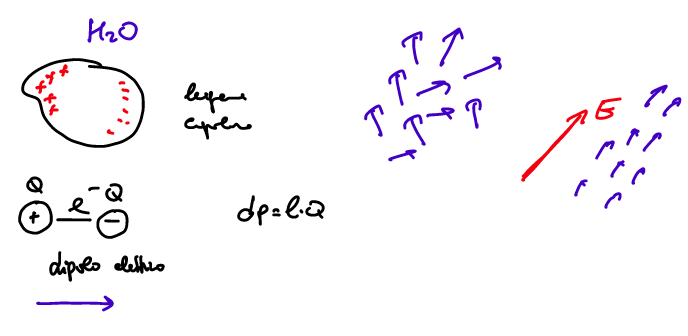
\includegraphics[scale=0.4]{immagini/pol_dip.png}
	\caption{Polarizzazione delle molecole a seguito dell'applicazione di un campo elettrico}
\end{figure}
\\\\Il mezzo viene quindi polarizzato per effetto del campo esterno.\\\\
\paragraph{Polarizzazione Ionica}
Nel corpo umano c'è tanta acqua, quindi è molto importante. Ci sono nel corpo altri materiali solidi, in cui è più difficile riconoscere la molecola in quanto sono organizzati sotto forma di reticolo, dove ogni nodo ha una composizione ionica e quindi una parte positiva ed una negativa ad esempio NaCl: l'Na si va ad "appiccicare" al Cl negativo.\\Nella singola cella, un pezzo è negativo ed uno è positivo, quando si applica un campo E, l'oggetto non può muoversi poiché vincolato, ma può essere deformato, quindi la poralizzazione ha effetto sulla modifica del reticolo, come riassunto nella figura sottostante
\begin{figure}[!h]
	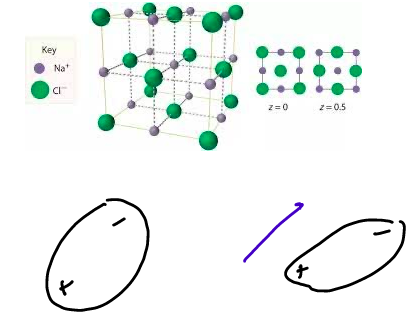
\includegraphics[scale = 0.5]{immagini/pol_io_effetti.png}
	\caption{Effetti della polarizzazione ionica}
\end{figure}
\paragraph{Polarizzazione elettronica}
Questa agisce direttamente sull'atomo, dove abbiamo il kernel positivo e la nube di elettroni. Anche in questo caso, in presenza di un campo E esterno la nube elettronica si può distribuire, su una forma magari più schiacciata, quindi abbiamo ancora un effetto dovuto allo stimolo esterno
\begin{figure}[!h]
	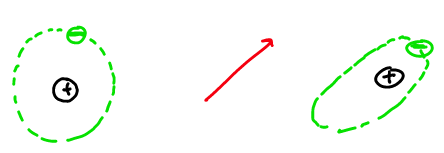
\includegraphics[scale=0.6]{immagini/pol_elettr_effetto.png}
	\caption{Effetti della polarizzazione elettronica}
\end{figure}
\\\\La dissipazione risulta nel momento in cui è necessario trasferire informazione, in quanto occorrono dei segnali sinusoidali, avremo che il campo esterno ha la seguente forma
\begin{figure}[!h]
	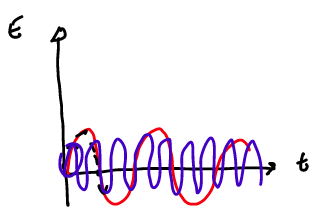
\includegraphics[scale=0.7]{immagini/appl_ce.png}
	\caption{Andamento nel tempo del campo elettrico generato da un segnale sinusoidale}
\end{figure}
\\\\questa applicazione di una forza elettrica alla struttura produce lavoro, siccome la materia vuole stare in un certo modo, la struttura tenderà ad opporsi allo stimolo e quindi ci sarà inerzia che produce attrito e che quindi conseguentemente verrà prodotto un riscaldamento.\\La dissipazione è quindi dovuta alla coesione complessiva dell'organismo che tende a non far muovere le molecole come vogliono.\\È simile a cosa accade con un forno a microonde: se metto del grasso non si cuoce bene, se lo metto in acqua questa cede il calore e lo fa riscaldare più velocemente.\\Se ci fosse una frequenza maggiore, ci sarebbe un ritardo in quanto il corpo umano ha del ritardo per capire che sta succedendo qualcosa e quindi le molecole sono sollecitate contro una forza, ci sarà quindi prima un po' di inerzia per cui ci vuole del tempo prima che la struttura si accorga che sta arrivando un fonte d'onda, ma finché se ne accorge arriva già il fronte negativo e quindi quello che avviene è che l'interazione con la materia è ridotta e concentrata sulla parte esterna.\\\\Occorre ora capire come rappresentare il corpo umano: si usa il modello di Debye, per cui abbiamo
\begin{equation}
	\dot{\epsilon} = \epsilon_{\infty} + \dfrac{\epsilon_s - \epsilon_{\infty}}{1 + j\omega \tau} 
\end{equation}
dove
\begin{itemize}
	\item $\epsilon_s$ è la costante statica (??)
	\item $\epsilon_{\infty}$è la costante ottima
	\item $\tau$ è il tempo di rilassamento, legato al tempo che serve alla molecola per sentire lo stimolo e tornare alla condizione iniziale dopo che lo stimolo è finito. È quindi il ritardo con cui viene seguito lo stimolo
\end{itemize}
Se rappresentiamo consideriamo una rappresentazione grafica:
\begin{figure}[!h]
	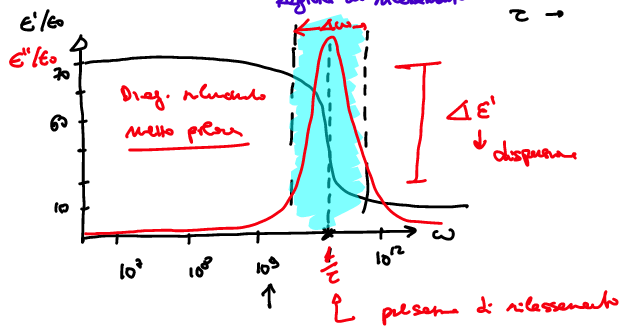
\includegraphics[scale=0.5]{immagini/eps_in_time.png}
	\caption{Andamento del rapporto $\frac{\epsilon'}{\epsilon_0}$ ed $\frac{\epsilon''}{\epsilon_0}$}
\end{figure}
\\\\teniamo conto che i GHz sono nell'ordine $10^9$, mettiamo ad $\frac{1}{\tau}$ la pulsazione di rilassamento.\\Avviene che la parte reale, quindi la capacità di immagazzinare energia e trasmetterla, in prossimità della frequenza in rosso ha un passaggio brusco, in un range di frequenza abbastanza stretto, la regione celeste che è la regione di rilassamento. La parte immaginaria ha un andamento totalmente opposto, in quella finestra c'è un assorbimento importante, le perdite sono elevate e quindi la potenza ceduta viene dissipata dal corpo. Questo è il digramma di rilassamento in un mezzo polare, le conseguenze da un punto di vista di comunicazione è nel che lavorare nella finestra celeste ci sono due fenomeni negativi:
\begin{itemize}
	\item molte perdite, se mando 1W di potenza buona parte del segnale è propagato;
	\item guardando alla permettività, mandando un segnale con una banda importante avrà ogni componente spettrale con una diversa velocità di propagazione e quindi avremo informazione dispersa
\end{itemize}
Quindi tutti i mezzi biologici sono dispersivi, quindi occorre lavorare distanti dalla zona di rilassamento perché il segnale ha effetti dispersivi e distorcenti.\\Visto invece dal punto di vista della fisioterapia, conviene lavorare in quella fascia perché c'è dissipazione e quindi riscaldamento.\\L'acqua ha una pulsazione di rilassamento dell'ordine di 20GHz, quindi il forno a microonde che funziona a 2450 MHz non è molto lontano.\\Questo avverrebbe se ci fossero solo composti polari come l'acqua, ma l'espressione quando consideriamo un corpo umano va adeguata a composti come proteine etc... ottenendo
\begin{equation}
	\dot{\epsilon} = \epsilon' - j \frac{\sigma}{\omega\epsilon_0} = \epsilon_{\infty} + \dfrac{\epsilon_s - \epsilon_{\infty}}{1 + (j \omega \tau)^{1 - \alpha}}
\end{equation}
(dove $0 < \alpha < 1$), 
ottenendo \textbf{l'espressione di Cole-Cole}.\\Mettendo tutto insieme, si è visto che tutto il corpo umano si può rappresentare con 4 di queste espressioni
\begin{equation}
	\dot{\epsilon} = \sum\limits_{i = 1}^{4} \dfrac{\epsilon_{si} - \epsilon_{\infty}}{1 + (j \omega \tau_i)^{1 - \alpha_i}} + \epsilon{\infty} - j \frac{\sigma_0}{\omega}
\end{equation}
dove tutti i parametri con la i e $\sigma$ sono dipendenti dai tessuti del corpo considerato.\\Rappresentando la finestra di dispersione, abbiamo 3 finestre per i vari parametri:
\begin{figure}[!h]
	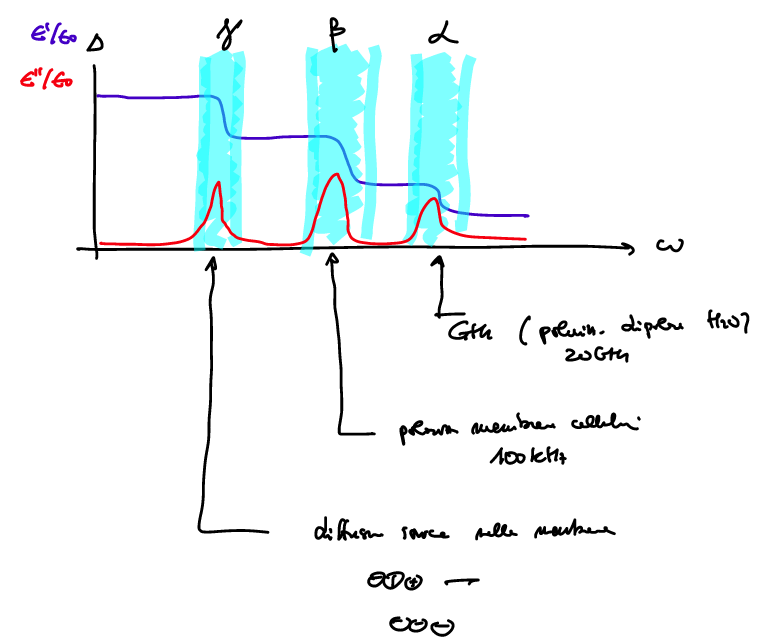
\includegraphics[scale=0.5]{immagini/fin_disp.png}
	\caption{Finestre di dispersione}
\end{figure}
\\\\nelle varie finestre ci sarà un incremento di perdite locale, questa è la risposta del corpo umano tessuto per tessuto (grasso, pelle, ...) in termini di riscaldamento, ed hanno nomi $\gamma$, $\beta$ $\alpha$, dove comandano diversi effetti
\begin{itemize}
	\item[$\gamma$] comanda la polarizzazione dipolare dell'acqua
	\item[$\beta$] comanda la polarizzazione delle membrane cellulari
	\item[$\alpha$] diffusione ionica nelle membrane
\end{itemize}
Immaginando di avere delle cariche libere: applicando il campo questi ioni entrano, poi applicandone un altro escono e quindi c'è assorbimento che produce delle perdite.
\subsection{Come caratterizzare i materiali}
Negli anni 90, sulla spinta dell'evoluzione della telefonia mobile, si è studiato l'impatto del telefono sulla testa e molti gruppi hanno studiato come caratterizzare i tessiti (sugli animali), usando l'espressione come interpolatore ed hanno estratto i parametri che sono di interpolazione. Ci sono dei DB dove in base alla frequenza ed al materiale c'è la lista dei parametri e quindi introducendola nella Cole-Cole generalizzata si ottiene la $\dot\epsilon$.\\Uno dei DB è Italiano, del CNR: niremf.ifac.cnr.it/emfref o /tissprop: si possono scaricare direttamente i parametri oppure avere i valori di permetività e conducibilità: otteniamo diversi valori tra cui la lunghezza d'onda ($\lambda = \frac{\lambda_0}{\sqrt[2]{\epsilon_r}}$). Prendendo ad esempio il muscolo, all'aumentare della frequenza, la conducibilità aumenta, la permettività diminuisce. Più c'è presenza di acqua, più permettività e conducibilità sono elevate.Ne riportiamo alcuni:
\begin{table}
    \begin{tabular}{c|c|c|c|c}
        Tessuto & 10 Mhz ($\frac{\epsilon_r}{\sigma}$) & 434 Mhz & 915 Mhz & 2450 Mhz\\
        \hline
        Grasso & 54 205 & 15 60 & 5 820 & 12 341\\
        Muscolo & 283 715 & 57 1120 & 55 1450 & 50 2272\\
    \end{tabular}
\end{table}
la differenza di conducibilità è importante, quindi il muscolo dissiperà sicuramente più potenza del grasso.
Cerchiamo ora di caratterizzare tutto da un punto di vista ingegneristico
\subsubsection{Assorbimento}
Un'onda arriva su un materiale: una grandezza importante è la densità di potenza dissipata nel corpo
\begin{equation}
	p_j = \frac{1}{2} \sigma \abs{E}^2
\end{equation}
e si misura in $\frac{W}{m^3}$.\\Per le norme di emissione si considera la SAR (Specific Absorption Rate), data da:
\begin{equation}
	SAR = \frac{p_j}{p}
\end{equation}
misurato in $\frac{W}{kg}$ e che indica quanta potenza viene assorbita per unità di massa del dispositivo, ed è quindi data da 
\begin{equation}
	\frac{\partial P}{\partial m} = \frac{1}{2\rho} \sigma \abs{E}^2
\end{equation}
e si usa in quanto è più facile da misurare.\\Se abbiamo un organo e vogliamo calcolare la potenza avremo quindi:
\begin{equation}
	P(\Omega_m) = \int\limits_{\Omega_m} P(r')SAR(r) dr'
\end{equation}
dove 
\begin{equation}
	SAR(\underline{r}) = \frac{1}{2 \rho(r)} \sigma(r) \abs{E(r)}^2 
\end{equation}
Le misure vengono fatte su dei "fantocci" che simulano le caratteristiche EM del corpo, il modo più semplice è usare acqua zucchero e sale:
\begin{itemize}
	\item l'acqua ha una permettività intorno a 70 Ghz
	\item il sale abbassa la $\epsilon_r$
	\item lo zucchero aumenta la $\sigma$
\end{itemize}
Ci sono delle ricette per ricostruire ogni organo e poter quindi misurare il SAR, altrimenti si usano fantocci da "macellaio", pezzi di carne etc...
\subsubsection{Propagazione nei tessuti biologici}
Consideriamo il caso più semplice possibile, dove il corpo umano è un mezzo omogeneo, avrà quindi una permettività $\epsilon' - j \frac{\sigma}{\omega}$.\\Immaginiamo di avere i due mezzi, (1) e (2) e che arrivi un campo elettrico che sia un'onda piana, si propaghi in direzione z, come mostrato in seguito:
\begin{figure}[!h]
	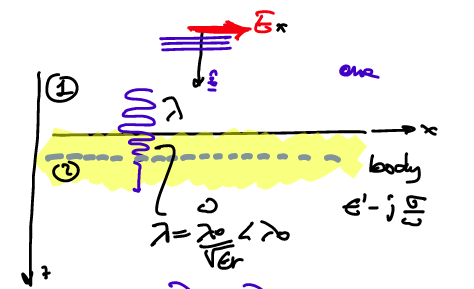
\includegraphics[scale=0.5]{immagini/es_propag.png}
	\caption{Esempio di propagazione di un'onda EM che attraversa due mezzi}
\end{figure}
\\\\Cosa accade al corpo: abbiamo, per un'onda piana
\begin{equation}
	E_x(z) = E_0 e^{-jkz}
\end{equation}
dove k è la costante complessa di propagazione
\begin{equation}
	k = \beta -j \alpha
\end{equation}
ed $\alpha$ e $\beta$ sono rispettivamente il fattore di propagazione ed il fattore di attenuazione:
\begin{equation}
	\alpha = \omega\sqrt[2]{\mu\epsilon'}\{ \frac{1}{2}[ \sqrt[2]{1 + (\frac{\epsilon^{\nu}}{\epsilon'})} -1] \}^{\frac{1}{k}}
\end{equation}
(esponente della quadra forse sbagliata).\\Sia $\alpha$ che $\beta$ dipendono dalla propagazione e dal mezzo.\\L'onda entra nel mezzo e man mano tenderà ad attenuarsi per via delle perdite, è importante capire da che punto in poi possiamo dire che l'onda si sia attenuata: definiamo $\delta_s$ = $\frac{1}{\alpha}$ ed è tale per cui z(profondità)= = $\delta_s$:
\begin{equation}
	\abs{\dfrac{E_x(\delta)}{E_y(\delta)}} = \frac{1}{e}
\end{equation}
che è circa del 37\%, quindi comunicare sotto questa soglia diventa molto complicato, la densità di potenza proporzionale al modulo di E si è ridotta invece del 13\%. Abbiamo un grafico come quello in \ref{sar_att}:
\begin{figure}[!h]
	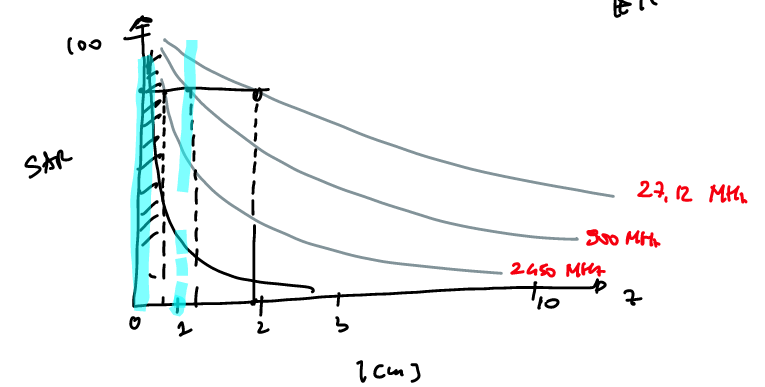
\includegraphics[scale=0.5]{immagini/attenuazione_sar.png}
	\caption{Attenuazione del SAR}
	\label{sar_att}
\end{figure}
\\\\supponiamo di fissare un valore di riferimento del SAR: questo sarà ottenuto nel mezzo, al variare della frequenza, ad una profondità via via crescente: se la profondità diminuisce lo spessore aumenta, quindi aumentando la frequenza otterremmo una profondità di penetrazione molto sottile.\\Fissando la profondità, all'aumentare della frequenza, il SAR tende ad abbassarsi quindi le conseguenze sono che volendo arrivare i profondità per comunicare con un dispositivo in profondità occorre usare frequenze basse, per cui il $\delta_s$ è basso, aumentando la frequenza l'interazione è sempre più in superficie \textbf{\textsf{(ricorda di smentire i coglioni che dicono che il 5G fa male perché entra nel corpo. COJONI, leggete le frequenze usate COJONI)}}.

\chapter{Lezione 3}
\section{Discontinuità fra due mezzi}
Cosa accade quando c'è una discontinuità: il corpo umano può essere rappresento in modo semplice come un mezzo non omogeneo, e quando l'onda incide il corpo umano sperimenterà una serie di effetti. Cosa accade quindi quando l'onda attraversa una superficie: consideriamo una superficie che separi due materiali differenti, materiale 1 e 2 ovvero grasso e muscolo: immaginiamo di avere determinati campi elettrici \underline{E} e di induzione \underline{D} e vediamo cosa succede alla potenza rilasciata sul corpo: la distribuzione della potenza dipende dall'incidenza dell'onda, possiamo avere campo elettrico paralleli o normale e dipendentemente dal fatto che il campo arrivi normale o parallelo avremo il \textbf{teorema di continuità dei campi}: a ridosso della discontinuità la componente tangente dei campi si conserva, quindi il campo parallelo sulla discontinuità $\pi$ si conserva senza avere salti, mentre la E$_\perp$ non si conserva, c'è un salto ma sappiamo che si conserva la componente D$_\perp$.\\Da queste considerazioni, cerchiamo di capire le conseguenze sulla distribuzione di potenza a ridosso delle superfici:
\begin{enumerate}
	\item Polarizzazione tangente:
	\begin{equation}
		\underline{E} = \underline{E_{\parallel}}
	\end{equation}
	avremo che 
	\begin{equation}
		P = \frac{1}{2}\sigma|E|^2
	\end{equation}
	e quindi le due P, una prima della superficie di separazione ed una dopo saranno 
	\begin{equation}
		p_1 = \frac{1}{2}\sigma_1|E_1|^2 p_2 = \frac{1}{2}\sigma_2|E_1|^2
	\end{equation} ne consideriamo il rapporto che sarà dato da
	\begin{equation}
		\frac{p_1}{p_2} = \frac{\sigma_1}{\sigma_2}
	\end{equation}
	\item Polarizzazione normale: ripartiamo da 
	\begin{equation}
		\frac{p_1}{p_2} = \dfrac{\frac{1}{2}\sigma_1|E_1|^2}{\frac{1}{2}\sigma_1|E_2|^2}
	\end{equation}
	dove le componente ortogonali NON sono più uguali come prima, quindi esprimiamo uno in funzione dell'altro: 
	\begin{equation}
		\epsilon_1 E_{\perp1} = \epsilon_2 E_{\perp2}
	\end{equation}
	ricaviamo $E_{\perp1}$ che messo nel rapporto fa si che questo dipenda anche dalla permettività:
	\begin{equation}
		\frac{p_1}{p_2} = \frac{\sigma_1}{\sigma_2} \abs{ \frac{\epsilon_2}{\epsilon_1}}^2
	\end{equation}
\end{enumerate}
Con degli esempi, CAPIAMO:\\ il mezzo 1 è grasso, mentre mezzo 2 è il muscolo. Fissiamo una frequenza fra quelle libere, f = 434 MHz e abbiamo $\epsilon_r$ e $\sigma$:
\begin{table}
	\begin{tabular}{|c|c|c|}
		& $\epsilon_r$ & $\sigma$\\
		muscolo & 60 & 1\\
		grasso & 15 & 0,1\\
		
	\end{tabular}
\end{table}
nella polarizzazione tangente, avremo che 
\begin{equation}
	p_f = \frac{1}{10} p_m
\end{equation} (dove f ed m sono fat e muscle), mentre nella nella polarizzazione ortogonale avremo 
\begin{equation}
	p_f = \frac{16}{10} p_m
\end{equation}
quindi si inverte: in un caso la potenza è maggiore nel muscolo, nell'altro caso nel grasso.\\Come sono gli andamenti:
\begin{figure}[!h]
	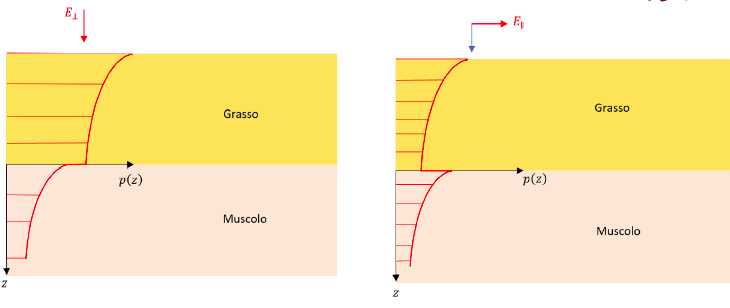
\includegraphics[scale=0.5]{immagini/disc_mezzi.png}
	\caption{Variazione di densità di potenza in base all'incidenza del campo E}
\end{figure}\\\\
la potenza man mano che si scende in profondità si attenua con legge esponenziale. Nel caso tangente, nella discontinuità, la potenza nel grasso è $\frac{1}{10}$ di quella nel muscolo, c'è un salto netto e poi continua a calare per via dell'attenuazione.\\Nel caso parallelo, c'è un salto ma in direzione opposta, perché in questo caso la potenza è maggiore nel grasso.\\L'effetto di assorbimento dei tessuti dipende quindi da come è fatto il dispositivo che genera il campo, in base a come lo genera: se normale, il valore nel muscolo è basso, mentre se parallelo è maggiore e quindi anche l'effetto di esposizione del corpo sarà differente.\\Vediamo ora l'effetto di questa potenza assorbita
\section{Effetti dell'assorbimento di potenza}
L'effetto principale è il riscaldamento ("effetto microonde"), quindi l'esposizione EM ha come effetto principale questo riscaldamento, che in alcuni casi come i sistemi terapeutici è voluto (sempre es. fisioterapia), in molti casi sono effetti collaterali, non voluti quindi si cerca di ridurli. Cerchiamo di capire il legame fra il SAR e la variazione di temperatura nel corpo: c'è l'equazione di Fourier che spiega come evolve un processo termico, che nel caso di una sorgente EM ha un pezzo in più
\begin{equation}
	\rho C \frac{\partial T(t)}{\partial t} = \Delta (K \Delta T) + p
\end{equation}
dove 
\begin{itemize}
	\item la temperatura T dipende da tempo e posizione (T(t, \underline{r}));
	\item $\rho$ è la densità (?)
	\item C è il calore specifico ovvero la quantità di calore assorbita da 1g di sostanza durante la variazione di temperatura di 1° ($\dfrac{J}{kgC°}$)
	\item K è il coefficiente di conducibilità termica
	\begin{equation}
		\frac{\Phi Q}{\Delta T} (\dfrac{W}{m°C})
	\end{equation}
	più k è elevato più il mezzo tende ad essere isolante. Infine p è la densità di potenza assorbita ($\frac{W}{m^3}$).\\ 
\end{itemize}
Ora, è molto più agevole considerare la stessa equazione quando dividiamo ambo i membri per $\rho$, in quanto
\begin{equation}
	\frac{P}{\rho} = SAR
\end{equation}
questo è il termine "forzante", questa diventa la sorgente del termine noto e quindi rilascia calore e tale potenza è una sorgente che si chiama \textbf{endogena}, in quanto è fornita all'interno del materiale mediante onda EM: se poggiamo un pezzo di metallo caldo su un oggetto, questa è una sorgente esogena, mentre questa si origina dall'interno.\\Nel corpo umano ci sono un paio di peculiarità:
\begin{itemize}
	\item è vivo, quindi si oppone a degli stress esterni, in questo caso il riscaldamento dell'onda EM col sangue che è un sistema di raffreddamento: il vaso si dilata ed il passaggio di sangue toglie calore. C'è un termine che si oppone al riscaldamento
	\item c'è poi un termine dovuto alla combustione chimica del cibo, che genera energia e si oppone
\end{itemize}
Otteniamo quindi la nuova equazione, Bioheat equation (Pennes 1948)
\begin{equation}
	\rho C \frac{dT(t)}{dt} = \Delta (k \Delta T) + p + M - B
\end{equation}
dove: 
\begin{itemize}
	\item M è il metabolismo ($\frac{W}{m^3}$), calore metabolico, \item B è la perfusione sanguigna, che ha segno meno perché tende ad opporsi per l'incremento dovuto agli altri termini.
\end{itemize}
Abbiamo che 
\begin{equation}
	B = W\cdot c_b (T - T_{arteria}
\end{equation}
dove T arteria se stiamo bene è di 37°, se questa diminuisce è il sangue che tende a scaldare, altrimenti raffredda. Ma dopo un po' c'è shock termico e quindi il tessuto comincia a bruciare: se ne vediamo l'andamento
\begin{figure}[!h]
	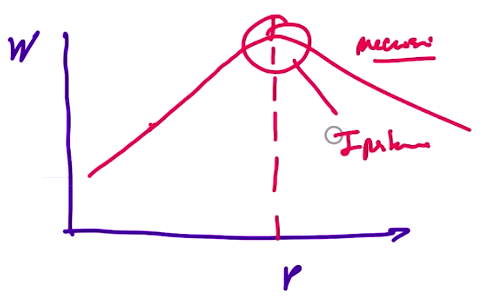
\includegraphics[scale=0.5]{immagini/andam_perf.png}
	\caption{Andamento della perfusione sanguigna, in funzione della densità di potenza}
\end{figure}

c'è un punto in cui va giù, ovvero quando la temperatura supera il 44° la perfusione sanguigna non ce la fa più perché il vaso non si più più estendere ed i tessuti necrotizzano (nel punto cerchiato si verifica l'ipertermia).\\Occorre quindi evitare che la temperatura inserita nel corpo dal dispositivo sia vicina ai 43°-44°, altrimenti si arriva a bruciare.\\Ci interessa l'equazione perché c'è un modo semplice per misurare il SAR: il cellulare rilascia un certo SAR nella testa, si parte dall'equazione di Pennes: il primo termine è istantaneo, poi c'è il termine di conduzione, la M quando c'è una sorgente esterna è piccolo rispetto al calore esterno ed anche la B è un fenomeno lento: il $\tau$ del fenomeno EM è veloce (ordine dei ns), se tocchiamo qualcosa di caldo non è istantaneo capire che si passa ad una temperatura fredda (ordine s), quindi applicando un fenomeno EM in un $\Delta t$ minore di un minuto nell'equazione rimane solo che 
\begin{equation}
	\rho C \frac{\partial T}{\partial t} \simeq p
\end{equation}
quindi dividiamo per $\rho$ ed otteniamo il SAR, che è proporzionale alla variazione di temperatura in un tempo abbastanza breve, quindi la posso approssimare come 
\begin{equation}
	C\frac{\Delta T}{\Delta t} \leq 1m
\end{equation}
Se mettiamo in una bacinella un liquido body-like (acqua zucchero sale) ed introduciamo un telefono cellulare, se facciamo una "foto" all'esterno (con termocamera o sondine), la zona sarà calda verso l'esterno e man mano sempre più fredda, così si può misurare il SAR prodotto dai dispositivi radianti.
\section{Normative EM}
Il progetto del dispositivo deve essere safety by design, quindi devo progettare prima il dispositivo che abbia fra i requisti una certa intensità di campo EM.\\Le attività del capire le soglie di esposizione nascono negli anni 80-90, l'impulso è stato dato dall'esplosione dei telefoni cellulari, c'è stato uno sforzo grande nel 97'-98' per capire quali parametri considerare e come caratterizzarli.\\Prima sono stati fatti degli studi con animali e tessuti espiantati e poi fatta una grossa analisi della letteratura scientifica. Sono stati poi fatti degli studi per cercare di correlare con le malattie (come tumori etc...), si è poi cercato di ridurre gli effetti accertati a breve termine, infine noti gli effetti gli studi si sono spostati sull'individuare le dosi soglia per evitare tali effetti.\\Ci sono due classi di effetti dell'esposizione ai campi EM:
\begin{enumerate}
	\item effetti diretti:
	\begin{itemize}
		\item accoppiamento con campi E a bassa frequenza
		\item accoppiamento con campi B a bassa frequenza
		\item assorbimento di energia EM.
	\end{itemize}
	Queste 3 tipologie di fenomeno producono due effetti percepibili:
	\begin{itemize}
		\item riscaldamento di organi e tessuti, ed è quella più facilmente quantificabile perché produce calore
		\item stimolazione di nervi e muscoli: c'è un disturbo dovuto al segnale, è possibile che il muscolo si contragga o che vengano stimolati degli effetti chimici e sono difficili da caratterizzare perché sono a lungo termine e sono più difficili da mettere in evidenza.
	\end{itemize}
	\item effetti indiretti, legati principalmente a
	\begin{itemize}
		\item alle correnti di contatto
		\item accoppiamento del campo EM con dispositivi impiantati, interazione con un dispositivo impiantato nel corpo. I primi pacemaker erano sensibili al telefono cellulare, sono stati poi protetti con dei filtri
	\end{itemize}
\end{enumerate}
Sull'analisi e la ricondizione degli effetti sono stati individuati dei limiti: inizialmente sono stati individuati i limiti di base, ovvero quelli legati alle grandezze EM che producono direttamente l'effetto, ovvero campo E nel corpo, al SAR ed in alcuni casi alla densità di potenza ovvero a grandezze direttamente generate nel corpo e che sono direttamente correlabili agli effetti diretti.\\Chiaramente cambiano in base alla frequenza, aumentandola, diminuisce la permettività sulla pelle.\\Misurarle è difficile, quindi sono stati introdotti degli \textbf{insiemi di livelli di riferimento o derivati}: sono delle grandezze che si possono valutare in assenza del corpo umano: se abbiamo un cellulare a contatto con la testa, leviamo la testa e calcoliamo le grandezze in un volume che sarebbe stato occupato dalla testa.\\Se scelti bene, rispettando i livelli di riferimento allora questi implicheranno che tali valori verranno rispettati anche quando sarà presente il corpo umano, MA NON vale il viceversa: se vengono rispettati i requisiti di base, non è detto che vengano rispettati quelli di riferimento.\\Le restrizioni di base sono quindi legate alla misurazione "in situ", mentre invece le restrizioni derivate sono misurate in assenza del corpo umano e quindi il loro rispetto implica i primi.\\Abbiamo ad esempio quelli per l'ELF fra 1-100 Khz
\begin{figure}[!h]
	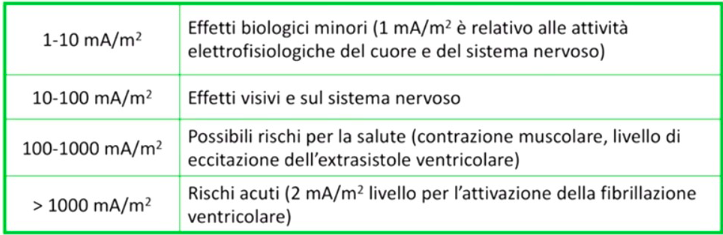
\includegraphics[scale=0.5]{immagini/elf_effetti.png}
	\caption{Effetti sul corpo umano in corrispondenza di Extremely Low Frequency}
\end{figure}
\\\\poi la microonde (100 Mhz in su), la sperimentazione animale indica come soglia di danno alla salute un incremento della temperatura di 1°C, per legarlo alla grandezza EM si è visto dalle misure che applicando un SAR per 6 min di 4 W/kg si innalza la temperatura di 1°C.\\I limiti di base del SAR sono diversi fra operatori e popolazione: un operatore può essere più esposto in quanto può prendere le dovute precauzioni, difatti per i lavoratori mediati su 6 min i valori sono circa 5 volte tanto, inoltre la media va fatta sui 10g: se ad un certo punto c'è un hotspot,  possibile superare il limite ma per un punto non posso buttare il dispositivo e quindi si fa una media su 10 g di materiale: si misurano i valori di SAR sui 10g e si fa questa media mobile così da buttare gli outlayers
\begin{figure}
	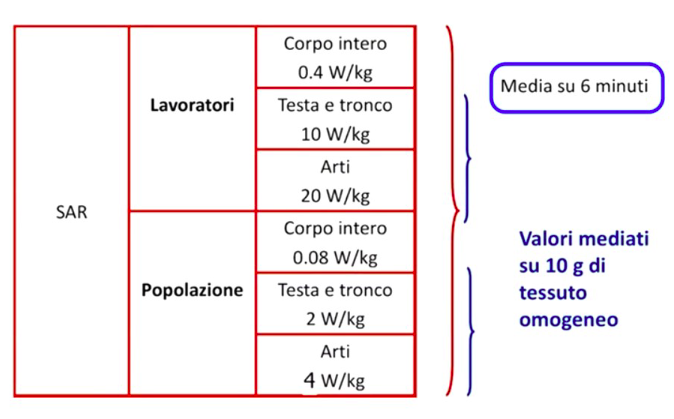
\includegraphics[scale=0.5]{immagini/limiti_sar.png}
	\caption{Limiti del SAR mediato su 6 minuti}
\end{figure}
\\\\Nel caso di dispositivi wearable, i limiti dei lavoratori sono coincidenti con quelli della popolazione\\Vi è poi un altro aspetto: le analisi vengono spesso fatte nel caso peggiore, ovvero quando viene trasmessa una sinusoide, quindi un segnale continuo.\\Nella realtà ogni dispotivo di telemetria ha un \textbf{duty cycle:} ci  sono parti alte e poi periodi di nulla, come mostrato in figura:
\begin{figure}[!h]
	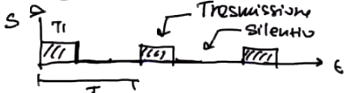
\includegraphics[scale=1.5]{immagini/duty_cycle.png}
	\caption{Trasmissione classica di un dispositivo di telemetria}
\end{figure}
\\\\Immaginiamo di avere un esempio in cui un dispositivo trasmette una volta l giorno lo stato di salute di una protesi impiantata, dove:
\begin{itemize}
	\item la trasmissione dura T = 1min;
	\item il SAR di picco è pari a 10 $\frac{W}{kg}$, quindi sopra soglia
\end{itemize}
averemo un minuto al giorno in cui il SAR è sopra soglia, ma facendo la media otteniamo 
\begin{equation}
	<SAR>_{6 min} = \frac{1}{6} \cdot 10 = 1,67 \frac{W}{kg}
\end{equation}
e quindi sotto la soglia di omologazione, avremo quindi un valore che è d $\cdot$ SAR.\\\\Se però un soggetto è portatore di oggetti come pacemaker i limiti vanno impostati per ogni istante di tempo: se viene messo in atto un attacco isico e si produce una potenza molto elevata, questo viene messo fuori uso.\\\\In Italia ed in Europa: il quadro italiano si pone in maniera molto restrittiva rispetto a quelle europee, dove in Europa sono indicati 40 V/m, in Italia ce ne sono 6. Inoltre, ovunque vanno rispettati certi valori, in siti come scuole etc.. ci devono essere valori ancora più bassi, inoltre a regime vanno rispettati dei valori ancora più bassi. La legislazione italiana fissa 3 livelli:
\begin{itemize}
	\item limite di esposizione: 20 V/m, non devono poter essere misurati in zone che non sono ad esempio dei tralicci recintati
	\item valore di attenzione: in alcuni ambienti dove ci si viva per un tempo maggiore di 4h consecutive non ci devono essere più di 6 V/m
	\item obiettivi di qualità: fare in modo che progressivamente in qualunque punto si vada verso i 6 V/m.
\end{itemize}
\subsection{Come fare una valutazione}
Ci si muove su tre livelli a complessità crescente:
\begin{enumerate}
	\item Misura del campo EM in assenza del corpo umano, andando a misurare i livelli di campo nel volume occupabile dall'uomo, si media per 6 min e si confrontano con i livelli derivati. Se rientrano nella normativa, possiamo omologare il dispositivo
	\item Se 1 da valori più elevati, occorre salire di complessità. Qui va fatta una simulazione EM, in cui si introduce il corpo umano, ma può andare bene un fantoccio di forme standard (cubi, cilindri), spesso di materiale omogeneo.\\Con un simulatore si simula il dispositivo e si calcolano campi e SAR nel fantoccio
	\item Se ancora i valori sono elevati, si fa una nuova simulazione con un modello antropomorfo, ovvero con tutti i tessuti del corpo umano con la sua permettività e conducibilità  e si valuta il SAR iterando ciascun componente del corpo umano.\\Se non si è conformi, tocca tornare alla progettazione.\\Esistono dei fantocci, il più famoso è visible human (progetto HUGO), un ergastolano che venne messo sotto gelatina, ghiacciato e fatto a fette e dopo la sedia elettrica venne "fotografato". È un fantoccio dove ci sono tutti i tessuti.
\end{enumerate}

\chapter{Lezione 4}
\section{Link bodycentrici - generalità}
Si fa riferimento a quei collegamenti nei quali in qualche modo compare il corpo umano, qui non solo c'è una sorgente che irradia, ma c'è un oggetto che si pone nel mezzo ed è molto complesso (corpo umano).\\Possiamo caratterizzare questi sistemi in base a 
\begin{itemize}
	\item[A)] orientamento della radiazione: immaginiamo di avere un corpo, possiamo avere un'antenna fuori che sta irradiando nel corpo oppure un'irradiazione che dal corpo irradia verso l'esterno.\\Possiamo quindi avere link:
	\begin{itemize}
		\item into the body, dove abbiamo ad esempio:
		\begin{itemize}
			\item sensori
			\item harvester: raccolgono l'energia esterna e la forniscono all'elettronica 
			\item sistemi di telemedicina: possiamo avere un dispositivo che cerca di interrogare dei sensori che sono all'interno del corpo
			\item terapia fisica, ovvero l'irraggiamento del corpo umano ai fini della terapia
		\end{itemize}
		\item out of the body (esterno), dove l'irradiazione dal corpo va verso l'esterno. Abbiamo:
		\begin{itemize}
			\item telemedicina, il sensore trasmette il dato verso l'esterno
			\item sensori
			\item trackers o beacon: dispositivi che servono per identificare la persona. Il dispositivo trasmette informazioni ad esempio sulla posizione
		\end{itemize} 
	\end{itemize}
	\item[B)] tipologia di interazione
	\begin{itemize}
		\item quasi statica, i campi E e B sono poco variabili nel tempo:
		\begin{itemize}
			\item induttivo, si lavora principalmente col campo B
			\item di tipo capacitivo, in cui si lavora col campo E 
		\end{itemize}
		\item zona di midfield, è una zona intermedia che domina molte delle applicazioni body centriche, non siamo più nel campo lontano ma non possiamo più separare campo elettrico e magnetico
		\item radiativa, abbiamo che i campi non sono più così separabili
	\end{itemize}
\end{itemize}
Immaginiamo di avere un elemento radiante, ed una corrente (antenna di cellulare, smartwatch etc...) ed avere r che è la distanza dominante: abbiamo 3 regioni
\begin{figure}[!h]
	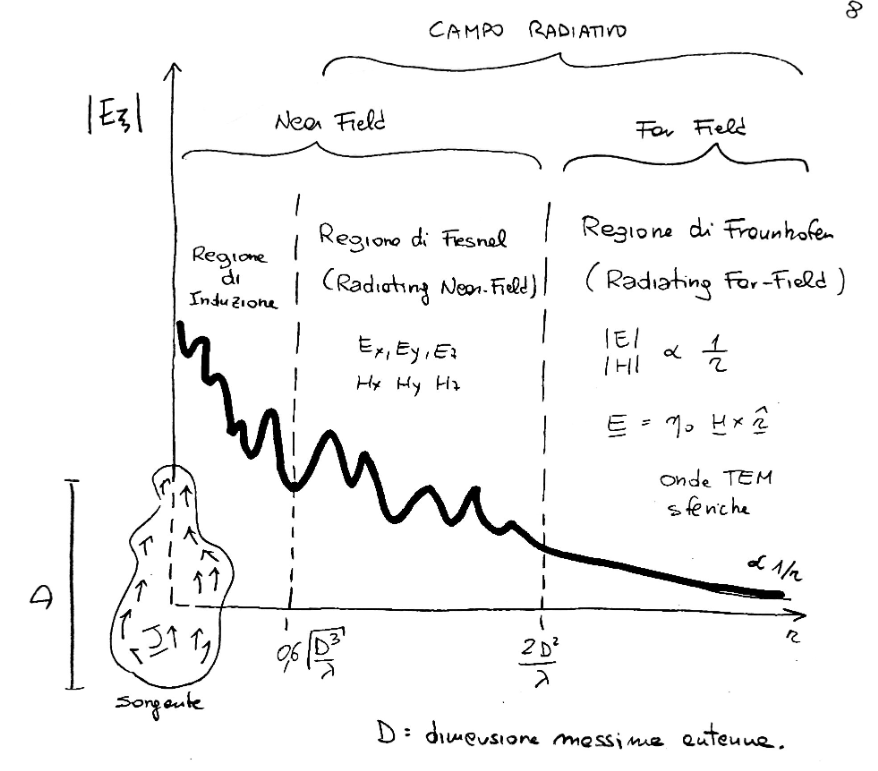
\includegraphics[scale=0.5]{immagini/regioni_campo.png}
	\caption{Regioni del campo radiativo}
\end{figure}
\\\\Nella zona di far field il campo elettrico e magnetico sono fra loro ortogonali, (anche a k che è la direzione di propagazione) e la densità di potenza è reale ed è proporzionale al campo elettrico, (copia tutte le formule)\\Nella zona induttiva, che è il near field, il campo varia molto lentamente e l'energia è induttiva(??) ma possiamo usarla per far colloquiare due dispositivi, ci sono tutte le componenti e sono mischiate e non si possono separare. Poi c'è la zona di mezzo dove comunque non si segue $\frac{1}{r}$.\\Va tenuto chiaro che: nelle zone vicine, quando abbiamo a che fare col corpo umano, c'è energia reattiva che  magnetostatica o elettrostatica che NON si propaga ma si può "raccogliere" ed accoppiare e quindi usare per le applicazioni.\\\\Un altro aspetto importante sono le frequenze di lavoro:
\begin{itemize}
	\item basse, Low Frequency ed High Freqeuncy (kHz - MHz), le LF vanno 30-300 KHz, mentre HF 2-30MHz. Sono tipiche dei sistemi quasi statici, quando lavoriamo con queste stabiliamo un regime quasi statico e quindi tutto interviene in campo quasi statico. Qui il campo si attenua di meno quando interagisce col corpo, lo spessore pelle è maggiore ma sono coinvolti dei dispositivi più grandi. Se volessi con una sola antenna trasmittente leggere tante antenne del corpo umano dovrei usare queste frequenza
	\item elevate, UHF e microwave. Le UHF sono 300 MHz - 3GHz, mentre le microvawe sono da 1 - 3GHz.  Sono tipiche dei sistemi radiativi. Penetrano meno, circa 4cm nel corpo e quindi possono interagire con la pelle meglio (penetrano meno) ma hanno come vantaggio di permettere l'utilizzo di antenne più basse.
	\item 
\end{itemize}
L'antenna è un oggetto poco miniaturizzabile, quindi in molti dispositivi l'ingombro è dovuto alla presenza di antenne (similmente a quanto accade per la batteria) soprattutto se l'antenna deve essere piccola.\\\\Altro aspetto importante sono le geometrie, i layout
\begin{itemize}
	\item in dispositivi quasi statici, abbiamo 
	\begin{itemize}
		\item coil, avvolgimenti nei sistemi magneto-statici
		\item piastre, che svolgono la funzione di condensatore
	\end{itemize}
	\item in sistemi radiativi abbiamo
	\begin{itemize}
		\item dipoli
		\item loop
		\item slot
		\item patch
	\end{itemize}
\end{itemize}
Seguono poi le tipologie di servizio, ovvero perché usiamo il sistema bodycentrico:
\begin{itemize}
	\item comunicazione: uno degli scopi principe.\\Sistemi wearable, con cui è possibile fare delle body area network. Ad esempio, in ambito militare, quando vanno in missione c'è una rete mash fra i vari soldati: ognuno ha una radio che permette di stabilire una comunicazione con gli altri fino ad arrivare al capo
	\item telemetrica e comando: abbiamo un dispositivo sul corpo o al suo interno, che deve mandare un messaggio all'esterno (telemetria). Il comando invece serve principalmente a configurare dei dispositivi impiantati: le pompe ad infusione, dispositivi che rilasciano farmaco, neuro-stimolatori periodicamente vanno controllate dagli esperti del settore (\textbf{\textsf{NON NOI}}).
	\item Wireless Power Trasnfer: trasferimento di energia per alimentare un dispositivo che non ha batteria o per evitare che la batteria di un dispositivo venga consumata per comunicare.\\Anche se un dispositivo medico non ha la batteria si cerca di non usarla i più possibile, quindi l'energia che serve per comunicare viene fornita dall'esterno.\\L'esempio classico è la ricarica del cellulare o dello spazzolino elettrico
	\item Marker / Labeling: alcuni dispositivi medici possono essere dei \textbf{marcatori}. I marker non trasmettono informazione, ma servono ad esempio per centrare il corpo umano rispetto a qualche altra sorgente.\\Il labeling è l'associazione al dispositivo medico un codice, simile al codice a barre, fatto a radiofrequenza da sistemi RFID quindi si può assegnare un identificavo ad un oggetto per leggere e scrivere dentro. Si fa quindi identificazione e tracking, ma anche localizzazione.
\end{itemize}

\subsection{Architetture di comunicazione}
Abbiamo due modalità per stabilire un link:
\begin{itemize}
	\item link simmetrici
	\item link asimmetrici
\end{itemize}
differiscono sostanzialmente nella gerarchia con cui uno trasmette ed uno riceve, c' è differenza nei protocolli usati, nella progettazione hadrware etc...

\subsubsection{Link simmetrici}
In un link in generale abbiamo due oggetti, A e B che devono scambiarsi delle informazioni.\\In un link simmetrico, possiamo definire trasmettitore TX e ricevitore RX: TX manda il segnale ed RX deposita tale segnale su un carico.\\È possibile anche che si scambino i ruoli fra i due ad un certo punto, quindi non parlano mai contemporaneamente (half duplex).
\begin{figure}
	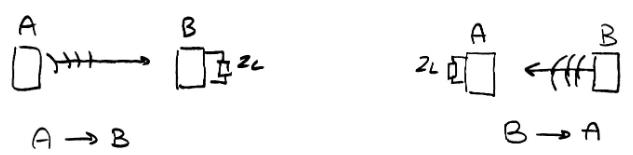
\includegraphics[scale=0.5]{immagini/com_halfd.png}
	\caption{Schema di comunicazione half duplex}
\end{figure}\\\\
L'esempio classico sono il cellulare che parla con stazione RB e poi altro cellulare, o anche i walkie talkie.\\Ambe due i dispositivi hanno la stessa elettronica e serve una fonte locale di alimentazione, quindi o una alimentazione ad un cavo fisico oppure una batteria.\\Esempi: bluetooth BT, che funziona a 2450 MHz, bluetooth BLE (low energy) che permette di avere una durata della batteria più lunga: la prima cosa da fare è il pairing fra i dispositivi.\\LTE (ex 4G), che è Long Term Evolution, 850-900 - 2100 MHz, ci sono i sistemi UMTS, CDMA, SCDMA\\Wi Fi, le cui frequenze sono 2450 - 5800\\5G, che ha diverse frequenze, 700 MHz, LTE, 3600Mhz, 26GHz fino a 60 GHz.\\Sistemi IoT: LoRa (Long Range) e SIGFOX: sono sistemi di Wireless Lan, sistemi con cui interconnettere oggetti e quindi molto usati in sistemi di IoT, possono collegarsi ad un hotspot tipo WiFi ma con range molto più alto e con batterie che durano molto tempo (ordine anni). Le frequenze sono più basse, 433 Mhz e 868 Mhz.

\subsubsection{Link asimmetrici}
Altra filosofia, che è molto gerarchizzata: tipicamente c'è un oggetto che si chiama lettore (Reader) che va ad interrogare un altro oggetto "stupido" da un punto di vista dell'elettronica e risponde per riflessione, quindi non ha sensori ma in qualche modo riflette il segnale modulandolo in modo da poter codificare i valori 0 ed 1. 
\begin{figure}
	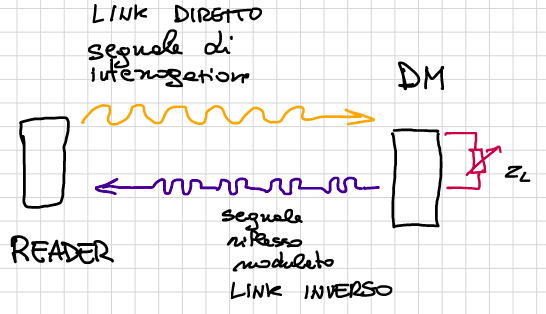
\includegraphics[scale=0.5]{immagini/com_fulld.png}
	\caption{Schema di comunicazione full duplex}
\end{figure}
Per farlo, c'è un interruttore del D che permette di modulare ma è molto semplice e non richiede batteria o elettronica complessa, tutta l'energia che serve per attivare l'interruttore arriva dal trasmettitore, a differenza invece del Reader.\\Ci sarà un link diretto dal lettore al trasmettitore e poi un link inverso che va dal dispositivo al reader.\\In questo caso i due dispositivi possono mandare segnali contemporaneamente, quindi con comunicazione full duplex. Abbiamo dispositivi monouso, come cerotti che evitano l'uso di batterie e costano meno.

\subsection{Efficienza dei collegamenti}
Quando si fa un collegamento, una delle cose più preziose è l'energia, in quanto sistemi wearable non possono essere collegati alla corrente e quindi tutta l'energia è data dalla batteria che non ha durata lunga, inoltre nel corpo umano si perde tanta energia per via delle perdite.\\Introduciamo in due step:
\begin{itemize}
	\item[1] solo antenna che trasmette in prossimità del corpo umano, ad esempio l'orologio che prova a collegarsi al wifi: abbiamo il corpo, un dispositivo che sta irradiando e che produce una radiazione che poi entra magari nel corpo.\\Consideriamo poi una superficie che racchiude tutto:
	\begin{figure}
		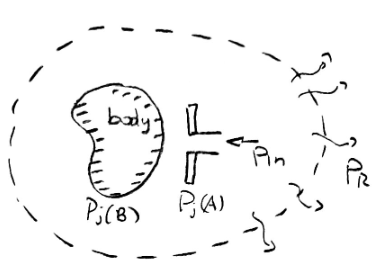
\includegraphics[scale=0.3]{immagini/eff_coll_1.png}
		\caption{Schema di trasmissione}
	\end{figure}\\\\
	potremmo applicare il thm di Pointying, abbiamo della potenza irradiata, della potenza dissipata nel corpo (P$_j$), quindi la potenza totale che fornisco è 
	\begin{equation}
		P_{in} = P_r + P_j(k) + P_j(B) + P_j(A)
	\end{equation}
	se abbiamo un sistema di comunicazione deve prevalere la potenza irradiata, mentre invece per sistemi che fanno terapia deve prevalere quella dissipata.\\\\Possiamo caratterizzare la bontà del trasmettitore in base alla efficienza 
	\begin{equation}
		\ni_R = \frac{P_R}{P_{in}} = \dfrac{P_r}{P_j(A) + P_j(B)} \equiv \dfrac{R_R}{R_R + R_j}
	\end{equation}
	abbiamo in più il termine (verde) che è proprio specifico della presenza del corpo.Si possono anche associare le resistenze delle antenne.\\Quando non c'è il corpo umano, la $R_R$ tende ad andare proporzionalmente come il raggio dell'antenna, l'andamento è simile a questo (metti immagine), le prestazioni migliorano ingrandendo l'antenna in modo da avere una resistenza di radiazione migliore ed enfatizzare quindi la parte radiata.\\Se abbiamo anche il corpo, aumentando le dimensioni dell'antenna irradia meglio ma manda più potenza nel corpo e ci sarà maggiore dissipazione. Se $\frac{R}{\lambda}$ aumenta abbiamo due effetti opposti:
	\begin{itemize}
		\item da una parte aumenta la resistenza di radiazione
		\item ma da una parte aumenta anche la resistenza di perdita
	\end{itemize}
	(copia ASSOLUTAMENTE L'IMMAGINE DEL DONDOLO)-\\Nei sistemi radianti, non comanda la lunghezza in se, ma la lunghezza RISPETTO alla lunghezza d'onda. Abbiamo il seguente andamento:\\ ad un certo punto, superato questo, il dispositivo irradierebbe come uno piccolo e quindi sarebbe poco efficiente.\\È un tradeoff e vale ogni volta che abbiamo un mezzo con perdite (pelle, pneumatico, etc...) l'effetto di portare un dispositivo in prossimità di un mezzo avrà un valore ottimale e tale valore ottimale dipende poco dalla forma dell'antenna (dipolo, loop, slot) ma tanto dalla forma: gli oggetti fatti a loop hanno una l$_{max}$ ottimale in termini di ingombro.
	\item[2] Consideriamo ora anche il link in presenza del corpo umano.\\Possiamo avere la seguente immagine:\\un'antenna che irradia, chiamiamo P$_l$ la potenza che verrà raccolta per far funzionare il dispositivo. Il parametro che descrive quanto p efficiente questo trasferimento di potenza dal tx all'oggetto è il PTE: $\frac{P_L}{P_{in}}$ e va massimizzato per avere un link efficiente.\\Dipenderà anche in questo caso dai tessuti, dalla posizione rispetto al corpo (più in profondità, maggiore l'attenuazione), dipende anche dalla forma delle antenne coinvolte ed ovviamente dalla frequenza (PTE tende a diminuire quando la frequenza aumenta perché l'attenuazione del corpo aumenta ed è quindi più difficile eseguire il comportamento).\\Possiamo scrivere $P_L = P_{in} \cdot PTE$, fissando la PTE, per aumentare la P$_L$ va aumentata la $P_{in}$, ma nel corpo aumenta anche il SAR ovvero la potenza rilasciata: qui il problema è che per aumentare la P$_L$ potremmo aumentare la potenza in ingresso ma se aumenta troppo il SAR sforo i limiti di legge e qui si capisce bene cosa vuol dire safety by design.\\Il primo anello della catena di progettazione deve:
	\begin{itemize}
		\item SAR $< SAR_{max}$
		\item P$_{in}$ < P max
	\end{itemize} 
	viene quindi fuori un vincolo per la PTE, imposto dal SAR: questo ci dice quindi quanto deve essere fatto bene il collegamento in modo da poter minimizzare la potenza necessaria.
\end{itemize}

\section{Link in near field}
Negli anni di fine 800 (1831) vengono fatti i primi studi da Faraday sulla induzione EM: gli studi avevano a che fare con due coil, in modo che questi potessero trasferirsi energia senza che questi si toccassero. L'accoppiamento veniva fatto mediante l'uso di materiale ferromagnetico, per molti anni venne usato ad esempio nei trasformatori ma non per la comunicazione.\\Agli inizi del 1900 ci sono gli esperimenti di Hertz e di Tesla, dove si parla proprio di trasmissione di informazione a distanza, Telsa introdusse anche i concetti di risonanza in quanto la sua ambizione era rifornire l'energia nelle città tramite una torre che mandava energia sulle case della città.\\Sono applicate nelle comunicazioni a bassa frequenza e piccola distanza, in ambito medico abbiamo dispositivi IMD (Implanted Medical Device) che possono essere pacemaker, defibrillatori, neurostimolatori etc... la comunicazione viene stabilita con un altro coil messo sulla superficie del body stabilendo un link a bassa frequenza. Sono link di tipo quasi statico, basati o su accoppiamento induttivo, o su accoppiamento induttivo risonante o accoppiamento capacitivo. Le frequenze di lavoro sono le HF ed LF, anche attorno ai KHz: in queste condizioni la capacità di conduzione del corpo è bassa, quindi basse perdite che permettono di avere PTE elevata, inoltre la permettività è elevata.\\I dispositivi non sono vere e proprie antenne, sono una specie di elettrodi in quanto lavorano in campo vicino.
\chapter{Lezione 5}
\section{Inductive (Magnetic) coupling}
Nell'accoppiamento siamo nel regime delle LF (125 KHz) e delle HF(13-56 MHz)
e possiamo usarlo per dispositivi medici impianti ma anche per la ricarica wireless.\\Tipicamente vengono usati due coil, di cui uno fa da trasmettitore ed uno raccoglie il campo vicino, siamo in campo vicino e non si può parlare di antenne:\\
\begin{figure}[!h]
	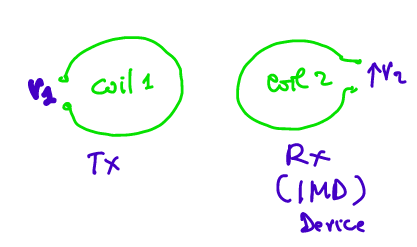
\includegraphics[scale=0.7]{immagini/spire.png}
	\caption{Coil usati per l'accoppiamento magnetico}
\end{figure}\\\\
abbiamo due spire ai capi della seconda spira vogliamo raccogliere la tensione.Parliamo di link induttivo perché avviene per induzione di Farady o magnetico perché avviene per il passaggio del campo da un coil all'altro, a noi interessa anche come sistema di comunicazione: questo sistema funzionerà come un trasformatore
 \\
 \begin{figure}[!h]
 	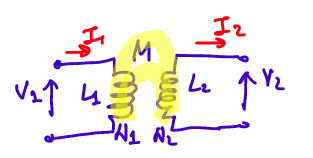
\includegraphics[scale=0.7]{immagini/trasf.png}
 	\caption{Sistema di comunicazione}
 \end{figure}\\\\
(M è il coefficiente di mutuo accoppiamento) ed abbiamo 
\begin{equation}
	\frac{V_1}{V_2} = \frac{N_1}{N_2}
\end{equation}
\begin{equation}
	\frac{I_1}{I_2} = \frac{N_2}{N_1}
\end{equation}
ed inoltre
\begin{equation}
	V_2 = -M \frac{dI_1}{dt}
\end{equation}
nel caso ideale abbiamo che tutto il flusso del primario è raccolto dal secondario e quindi vale:
\begin{equation}
	M = \sqrt{L-1 \cdot L_2}
\end{equation}
nel caso reale invece abbiamo:
\begin{equation}
	M = k \sqrt{L-1 \cdot L_2}
\end{equation}
dove k è il \textbf{coefficiente di accoppiamento}, e vale k $\in [0,1]$.\\
Vogliamo vedere come esprimere M per il sistema di due coil che sarà poi quello che legherà la tensione nel device rispetto alla tensione accesa nel primario:\\se c'è un filo lineare percorso da una corrente I\\
\begin{figure}[!h]
	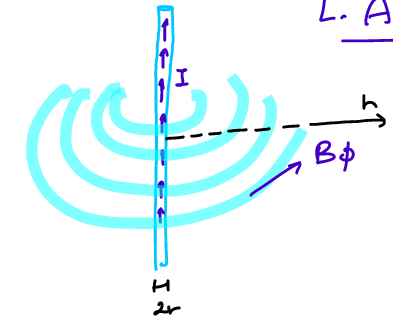
\includegraphics[scale=0.6]{immagini/corrente_filo.png}
	\caption{Campo magnetico generato da un filo lineare}
\end{figure}\\\\
viene generato un campo magnetico e dalla \textbf{legge di induzione di Ampere} abbiamo
\begin{equation}
	\underline{B} = \frac{\mu_0 I}{2 \pi r}\Phi
\end{equation}
se "curviamo" questo filo otteniamo questa configurazione
\begin{figure}[!h]
	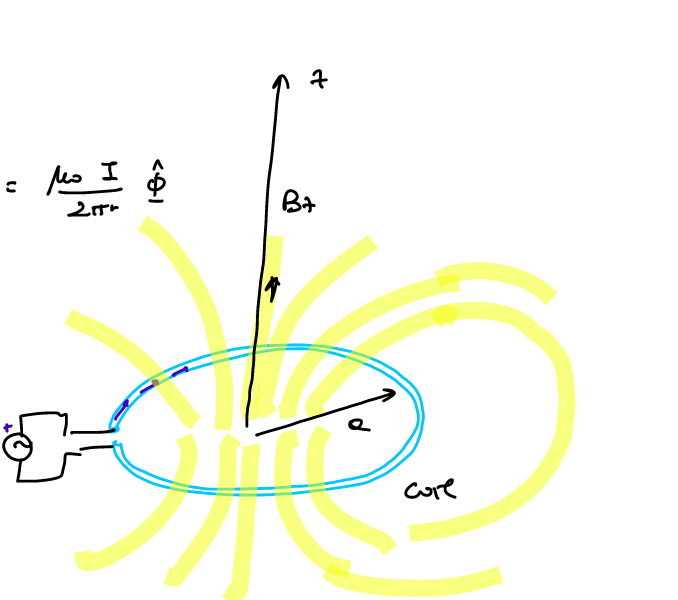
\includegraphics[scale=0.6]{immagini/solen.png}
	\caption{Campo magnetico generato da un filo lineare curvato}
\end{figure}
mettiamo un generatore in modo che scorra una corrente nel verso mostrato, allora verrà generato un campo magnetico le cui linee di forza sono come mostrate, considerando la $B_z$ che sarà
\begin{equation}
	B_z = \frac{\mu_0 I a^2}{2(a^2 + r^2)^{\frac{3}{2}}}
\end{equation}
se supponiamo di avere N spire, l'espressione precedente viene moltiplicata per N.\\Si vede intanto che se la distanza è r $>>$ a, allora $(a^2 + r^2) \approx r^2$, quindi avremo un andamento come $\frac{1}{r^3}$ e quindi il campo più forte si avrà nelle vicinanze ed avremo che $B_z$ si può approssimare con
\begin{equation}
	B_z = \frac{\mu_0 NI a^2}{2}\frac{1}{r^3}
\end{equation}
\\\\Consideriamo ora due coil, uno che trasmette ed uno che riceve \\
\begin{figure}
	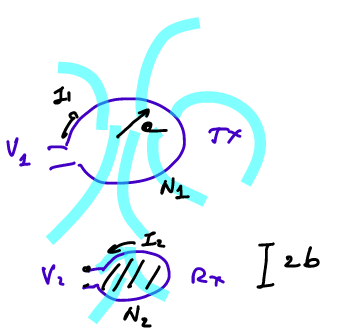
\includegraphics[scale=0.6]{immagini/coils.png}
	\caption{Sistema di due coil (tx ed rx)}
\end{figure}
\\\\avremo che RX concatenerà alcune delle linee del campo magnetico e quindi vale la \textbf{legge di Faraday}, che dice che un campo magnetico B variabile nel tempo che concatena una spira chiusa andrà ad indurre una ELF (Forza Elettromotrice Indotta) (vedi bene).\\Se consideriamo il flusso $\phi$ del campo magnetico:
\begin{equation}
	\phi(t) = \int\int \underline{B}(t) \cdot d\underline{s}
\end{equation}
allora la EMF sarà 
\begin{equation}
	V_2 = -N\frac{d\phi}{dt}
\end{equation}
c'è un meno perché la tensione che viene indotta ai capi nel secondario a sua volta tende a muovere degli elettroni che genera un campo magnetico che si oppone al primo (altrimenti si violerebbe il principio di conservazione).\\La applichiamo al nostro caso:
\begin{equation}
	V_2 = -N_2 \frac{d}{dt} \psi_{2,1} = -N_2 \frac{d}{dt} \int\int\limits_{S_2} \underline{B_1} da
\end{equation}
dove il pedice a destra è la causa, quello a sinistra è l'effetto (coil 2, coil 1), sostituiamo poi l'espressione per B (supponendo che i due coil siano colinerari, quindi allineati rispetto a z) ottenendo:
\begin{equation}
	V_2 = -N_2 \frac{d}{dt} \int\int\limits_{S_2} \frac{\mu_0 I_1 a^2 N_1}{2(a^2 + r^2)^{\frac{3}{2}}} da
\end{equation}
supponendo che i coil siano piccoli, possiamo considerare che il campo sia costante sul coil, possiamo integrare e moltiplicare per l'area:
\begin{equation}
	V_2 = -[] \frac{dI}{dt}
\end{equation}
e la confrontiamo con la $V_2$ ottenuta dalla precedente, quindi M è $f(N_1\cdot N_2, b^2, \frac{1}{r^3})$.\\\\Cosa succede invece se il TX e l'RX non sono allineati: supponiamo di avere un angolo $\alpha$ fra i due assi, il secondario raccoglierà meno flusso e quindi possiamo tenere conto della mutua rotazione con un cos($\alpha$), ottenendo un'espressione più completa di M aggiungendo il cos($\alpha$)
\begin{equation}
M = 	\dfrac{\mu_0 I a^2 N_1}{2(a^2 + r^2)^{\frac{3}{2}}} \pi b^2 cos\alpha
\end{equation}
\\\\Per incrementare il trasferimento di potenza fra un coil e l'altro possiamo:
\begin{enumerate}
	\item aumentare l'intensità del campo \underline{B}, ma viene limitato dai limiti del campo a basse frequenze
	\item possiamo diminuire la distanza fra tx ed rx, ma non è una cosa che si può fare sempre, ad esempio per un dispositivo medico impiantato
	\item aumentare la frequenza del campo \underline{B}, in modo che l'attenuazione sia meno evidente. La derivata nel dominio armonico è un -j$\omega$ ma l'aumento della corrente ha delle contro-indicazioni. Abbiamo $\frac{dI}{dt}$ $\rightarrow$ -j$\omega$I (quindi $V_2$ aumenta) ma questo fa si che ci siano più perdite e si dissipi di più (più potenza)
	\item aumentare il flusso concatenato, ovvero fare in modo che il secondario raccolga più possibile del primario che tipicamente si ottiene facendo in modo che il primario ed il secondario abbiano le stesse dimensioni oppure facendoli lavorare per \textbf{risonanza}.\\Anche qui occorre fare i conti con le normative di esposizione
\end{enumerate}
\subsection{Accoppiamento induttivo risonante}
Uno dei modi è quindi fare un'accoppiamento induttivo risonante: si deve a Telsa, alla risonanza si ha tipicamente un massimo trasferimento di potenza (o quanto meno di stimolo).\\Per far risonare i due sistemi occorre, innanzi tutto fare in modo che il tx sia risonante: occorre agire sulle dimensioni in modo che la parte immaginaria x sia pari a 0.\\Sull'RX c'è poco margine, se abbiamo un loop piccolo e ne vediamo la reattanza in ingresso $X_{in}$ se 2$pi$B << x allora la reattanza sarà induttiva, ovvero $>$ 0 e si comporterà come un circuito.\\Ci sarà poi il carico del dispositivo, ovvero qualcosa che gli permetta di utilizzare l'energia, occorre aggiungere un condensatore che può essere messo sia in serie che in parallelo.\\Avremo quindi il coil trasmittente e possiamo mettere in risonanza sia tramite un condensatore in serie oppure con un condensatore in parallelo 
\begin{figure}[!h]
	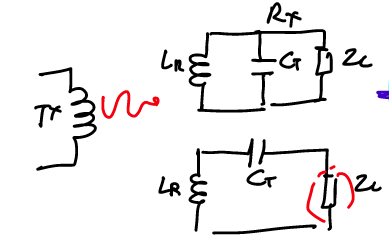
\includegraphics[scale=1]{immagini/cond_ser_parall.png}
	\caption{Condensatore in parallelo o in serie per il ricevente}
\end{figure}
 entrambe danno la stessa potenza sul carico ma cambiano i valori mutui di corrente e di tensione:
 \begin{itemize}
 	\item lo schema in parallelo darà corrente bassa e tensione elevata
 	\item lo schema in serie il contrario
 	tipicamente si sceglie il parallelo: dopo il carico, c'è tipicamente un rettificatore AC$\rightarrow$DC e poi deve esserci un convertitore da corrente alternata a corrente continua per alimentare la circuiteria digitale (l'elettronica).
 \end{itemize}
Questo tipo di dispositivo lavora meglio con alte tensioni, quindi si preferisce usare uno schema parallelo.\\\\Abbiamo quindi il nostro modello circuitale TX ed RX:
\begin{figure}
	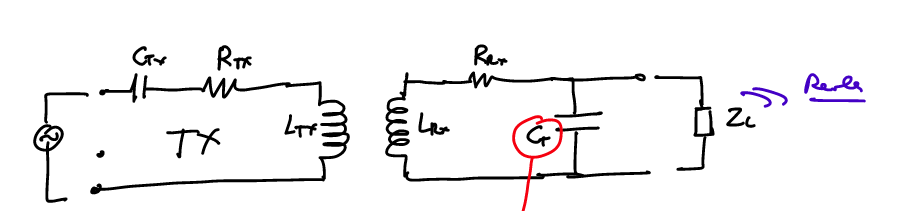
\includegraphics[scale=1]{immagini/schema_circuitale.png}
	\caption{Schema circuitale di TX ed RX}
\end{figure}
dove nel ricevitore C$_T$ è il condensatore di tuning. La $C_T$ va scelta in modo tale che 
\begin{equation}
	f_0 = \frac{1}{2\pi\sqrt{L_{R_x} \cdot C_T}}
\end{equation}
Abbiamo trovato che
\begin{equation}
	V_2 = -N_2 \frac{d}{dt} \int\int\limits_{R} \underline{B} ds
\end{equation}
passando al dominio dei fasori, sappiamo che $\frac{d}{dt} = j\omega$ ed abbiamo quindi 
\begin{equation}
	V_2 = -N_2 j\omega B_0 S_{RX} cos\alpha Q_{RX}
\end{equation}
in più compare il fattore di qualità Q del ricevitore, dove è definito come 
\begin{equation}
	Q_{RX} = \omega \frac{\Xi_{RX}}{P_{j, RX}}
\end{equation}
Più Q è elevato e meno potenza dissipata ci sarà e quindi più quella che viene immagazzinata.\\Per fare quindi in modo che aumenti $V_2$ occorre avere un fattore di qualità elevato che si ha quando il sistema è risonante, ancora di più se in parallelo.\\Avere un Q elevato comporta una criticità operativa, ovvero la banda è stretta in quanto la larghezza di banda è 
\begin{equation}
	B \propto \frac{1}{Q}
\end{equation}
(quanto più è alto il fattore di qualità tanto più c'è sensibilità a spostamenti dalla frequenza di lavoro).\\\\Con la $V_2$, quando questa è maggiore di una tensione di threashold che è connesso al coil primario, il secondario si accende e comincia a funzionare, quindi $V_2$ deve essere $> V_{th}$ e fissata la distanza sappiamo quali sono il fattore di qualità da avere etc... che sono valori minimi.\\Un parametro di performance che ci interessa è la \textbf{PTE (Power Trnasfer Efficiency)}, definita come 
\begin{equation}
PTE = \frac{P_L}{P_{in}}	
\end{equation}
quindi la 
\begin{equation}
	(1-PTE)P_{in}	
\end{equation}
è quella persa.\\È stato trovato che la PTE è data da:
\begin{equation}
	PTE = [1 + \frac{1}{q} + \dfrac{1}{M^2 Q_{TX} + Q_{RX}}(2 + q + \frac{1}{q})]^{-1}
\end{equation}
 \textbf{IMPORTANTE: QUESTO GROSSO GOAT DI MARROCCO TI FA PORTARE IL FORMULARIO (KING)}), dove q è dato da:
\begin{equation}
	q = \sqrt{\dfrac{1 + M^2\cdot Q_{TX}\cdot Q_{RX}}{1 + M^2 \cdot Q_{TX} Q_{RX}^{-1}}}
\end{equation}
e vale per un circuito risonante parallelo.\\Nota importante: a frequenza basse (dove siamo) le perdite dei tessuti sono basse, cioè la conducibilità $\sigma$ (legata alle perdite) è piccola. Siamo nell'ordine dei 100KHz e contano quasi più le perdite sui conduttori che sul tessuto.\\Tipicamente quindi i due coil conviene farli di dimensioni simili in modo che buona parte del campo B prodotto dal primario viene raccolto dal secondario, in alcuni casi però non è possibile farli simili perché magari un coil ricevente deve poter raccogliere più coil tx, quindi è possibile usare un coil booster:\\
\begin{figure}
	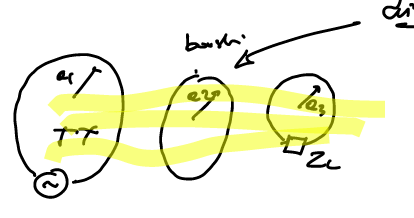
\includegraphics[scale=1]{immagini/booster_coil.png}
	\caption{Sistema con coil booster}
\end{figure}
\\\\
il booster ha dimensioni intermedie fra i due, è a corto circuito ed ha l'effetto di ridirezionare il flusso verso coil più piccoli.\\Funziona come un \textbf{direttore di antenna}, in modo che se il coil è piccolo ed in un posto difficilmente raggiungibile possiamo usare un coil intermedio in modo che venga ridirezionato il flusso fino a dove serve.
\subsection{Criticità}
Principalmente legata la disallineamento: immaginiamo di avere la classica stratificazione, col dispositivo IMD (copia disegno)\\l'ideale sarebbe avere il coil che trasmette in un certo punto, ma una volta impiantato non posso più vederlo, per cui se abbiamo un disallineamento non concateno più il massimo del campo e quindi avremo un notevole decadimento delle prestazioni.\\Una soluzione è porre dei magneti con opportune polarità in modo che il campo prodotto di polarizzazione fra i due magneti vada a far allineare i coil, quindi si possono impiantare dei micromagneti sotto pelle sia sul tx che sull'rx\\Altra criticità è la flessibilità: in molte applicazioni, soprattutto quando il dispositivo deve aderire a delle protesi o a degli organi, viene realizzato con un'elettronica flessibile, si può realizzare su delle membrane.\\Immaginiamo di avere il coil "spalmato" su qualcosa che può flettersi, ma questo provoca un cambiante nella forma che provoca un detuning: cambia il fattore di qualità e si abbassa la tensione raccolta.\\L'oggetto va quindi progettato a priori per quelle condizioni.\\Ultimo punto, riguarda i materiali.Essendo a frequenze basse, le perdite sui conduttori pesano e quindi servono conduttori con perdite basse come il rame, che però non è biocompatibile. Oggetti biocompatibili sono il titanio, che non è però un buon conduttore (1.5 ordini in meno del rame) e quindi tende ad avere perdite maggiori.\\Si può usare il rame andando a fare un coating, ovvero un rivestimento del conduttore di rame con materiale biocompatibile, come ad esempio
\begin{itemize}
	\item silicone
	\item materiali ceramici, che vanno bene per dispositivi solidi
	\item poliammide (PEEK il più usato, polimero semi cristallino), sono polimeri ovvero materiali fatti da tanti monomi agglomerati che formano una matrice molto solida
	\item zirconia
\end{itemize}


\subsection{Comunicazione del ricevitore col trasmettitore (modulazione capacitiva)}
Per la comunicazione inversa si può usare un link simmetrico, quindi si invertono le parti oppure si usa un link asimmetrico (come si tende a fare sempre di più) cioè il ricevitore va a modificare l'accoppiamento col trasmettitore ovvero fa quella che si chiama una \textbf{modulazione capacitiva}: si fa in modo che il sensore vada con una logica binaria a modificare l'accoppiamento col primario così che questo si renda conto che qualcosa sta irradiando dall'altro lato.\\Consideriamo il circuito di prima:\\
\begin{figure}[!h]
	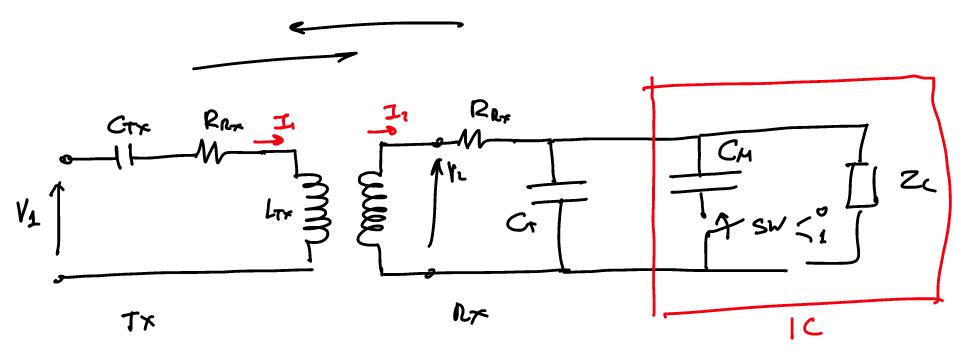
\includegraphics[scale=0.5]{immagini/schema_mod_cap.png}
	\caption{Schema per la modulazione capacitiva}
\end{figure}
\\\\
abbiamo poi un altro pezzo, una scatola dove troviamo un altro condensatore che si può connettere / sconnettere con interruttore (sarà il condensatore di modulazione) e quindi sarà il blocco che esegue tale modulazione, sarà un circuito integrato.\\Lo switch ha due stati, 0 o 1 (chiuso aperto) ed in base a questo il $V_1$ vedrà una cosa o un'altra:
\begin{itemize}
	\item switch open: bit '0', $V_1$ sarà dato (risolvendo il circuito) nel dominio dei fasori 
	\begin{equation}
		V_1 = \frac{1}{j \omega G_X} I_1 + j \omega L_{TX}I_1 + R_{TX}I_1 - j\omega M I_2^{(0)}
	\end{equation}
	e dove la frequenza è pari alla frequenza di risonanza
	\begin{equation}
		f_0 = \frac{1}{2\pi \sqrt{L_{RX} \cdot C_T}}
	\end{equation}
	abbiamo poi che il circuito è risonante e quindi il valore visto è alto, perché l'accoppiamento è forte.\\Ripuliamo quindi i termini reattivi in quanto siamo in risonanza
	ottenendo
	\begin{equation}
		V_1^{(0)} = R_{TX}I_1 - j\omega M I_2^{(0)}
	\end{equation}
	\item switch close: bit '1', abbiamo la somma dei due condensatori, di tuning e di modulazione e quindi avremo una $f_1$ diverso dalla frequenza di risonanza:
	\begin{equation}
		f_1 = \frac{1}{2\pi \sqrt{L_{RX}(C_T + C_M)}} \neq f_0
	\end{equation}
	 I due coil quindi non si parlano bene perché non sono in risonanza e quindi la $V_1$ vista dal primario sarà bassa
	 \begin{equation}
	 	V_1^{(1)} = R_{TX}I_1 -j\omega MI_2^{(1)}
	 \end{equation}
\end{itemize}
governando lo switch secondo elettronica digitale (apri/chiudi) facciamo in modo che $V_1$ sia modulato in ampiezza in quindi ottenere una situazione di questo tipo: vogliamo mandare questa stringa, sul writer si vedrà un qualcosa del genere:\\
\begin{figure}[!h]
	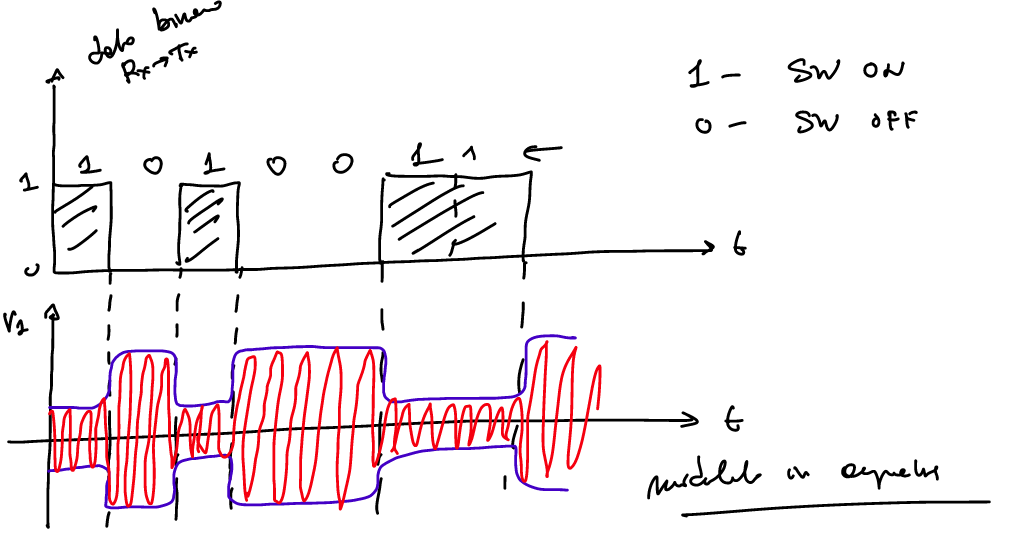
\includegraphics[scale=0.5]{immagini/rx_verso_tx.png}
	\caption{Segnale di risposta del ricevente}
\end{figure}\\\\
dove abbiamo il segnale modulato in ampiezza.\\Questo è il sistema con cui funzionano i sistemi NFC.\\È il primo collegamento in campo vicino visto, usato sia in ambito medico che anche in campo logistico, basato su coil:
\begin{itemize}
	\item patenti
	\item codice fiscale
\end{itemize}
tutto funziona esattamente così.


\chapter{Lezione 6}


\section{Near-field: link capacitivi}
Sono dei link meno usati degli altri ma hanno dei risvolti interessanti. Lavorano a frequenze un po' più alte, sui pochi MHz, ma se le dimensioni sono piccole si può anche arrivare al GHz.\\Immaginiamo un condensatore a facce piane e parallele, immaginiamo che sia alimentato da un generatore \\
\begin{figure}[!h]
	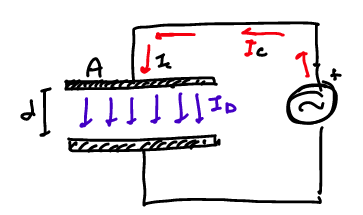
\includegraphics[scale=0.7]{immagini/circ_cap_link.png}
	\caption{Esempio di circuito}
\end{figure}\\\\
la corrente gira sul filo, il circuito ha un interruzione ma la corrente circola poiché viene generata una corrente di spostamento fra le facce del condensatore (legata al campo che si propaga e che carica il condensatore).\\La $I_d$ sarà
\begin{equation}
	\epsilon_0 \epsilon_r A \frac{\partial\underline{E}}{\partial t}
\end{equation}
oppure nel dominio dei fasori
\begin{equation}
	j\omega \epsilon_0\epsilon_rA\underline{E}
\end{equation}
Possiamo immaginare di avere il condensatore a cavallo del corpo umano, così, da poter mandare un'informazione alla piastra dentro.\\Si divide il condensatore a metà, su ogni faccia di esso, collegandola come segue
\begin{figure}[!h]
	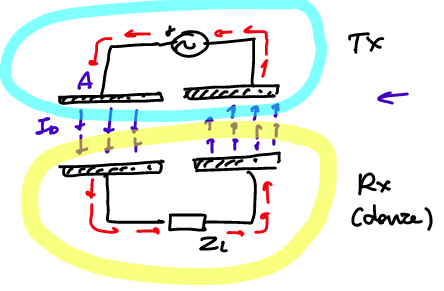
\includegraphics[scale=0.5]{immagini/divisione_circ.png}
	\caption{Divisione del circuito}
\end{figure}
le correnti faranno lo stesso giro di prima, abbiamo quindi due oggetti separati:
\begin{itemize}
	\item il primo è fatto con le due metà della prima faccia, sarà il tx
	\item il secondo è fatto dalle due metà dell'altra, sarà per noi il rx
\end{itemize}
il dispositivo deve quindi avere due elettrodi belli larghi che userà per accoppiarsi elettrostaticamente con i due elettrodi del ricevente.\\L'accoppiamento come detto è principalmente elettrostatico, quindi domina il campo E.\\Occorre però fare attenzione:
\begin{figure}[!h]
	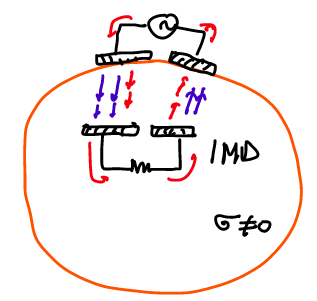
\includegraphics[scale=0.6]{immagini/circ_divis_corpo.png}
	\caption{}
\end{figure}
fra le due coppie di armature non abbiamo solo la corrente di spostamento, il mezzo corporeo ha una conducibilità $\neq 0$, quindi ci saranno anche delle correnti di conduzione che sono legate al fatto che il materiale permette di spostare anche elettroni.\\Nuovamente ci sono due fenomeni contrastanti:
\begin{itemize}
	\item propagazione, legato alle correnti di spostamento;
	\item dissipazione, legato alle correnti di conduzione.
\end{itemize}
Cerchiamo di caratterizzare le due entità:
\begin{itemize}
	\item $I_d = \epsilon_0 \epsilon_r A \frac{\partial\underline{E}}{\partial t}$
	\item la corrente di conduzione è data dalla legge di Ohm: abbiamo il body \\
	\begin{figure}[!h]
		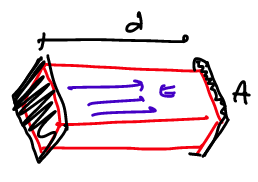
\includegraphics[scale=0.7]{immagini/rapp_body.png}
		\caption{Rappresentazione di un blocchetto di corpo}
	\end{figure}\\\\
	la resistenza del blocchetto è $R = \frac{1}{\sigma} \frac{d}{A}$, quindi $I_c = \frac{V\sigma(\omega)A}{d}$
\end{itemize}
come facciamo ad enfatizzare la corrente di spostamento:
\begin{itemize}
	\item se aumentiamo il campo E:
	\begin{itemize}
		\item possiamo aumentare la $V_0$ del generatore, ma se il campo aumenta dobbiamo fare attenzione ai limiti di esposizione
		\item ridurre d, ovvero la distanza fra le due armature così che il campo sia più intenso. Ma ci sono delle limitazioni legate all'istallazione
		\item aumentare l'area A delle placche (degli elettrodi), anche qui un punto di attenzione è l'ingombro per dispositivi impiantati
	\end{itemize}
	\item incrementare la frequenza, poiché la $I_d $pro a $j\omega$ (che è la derivata rispetto al tempo nel campo dei fasori), ma l'aspetto critico sono le perdite nei tessuti
\end{itemize}
Per ridurre la $I_c$ occorre fare l'opposto di quello che si faceva prima:
\begin{itemize}
	\item ridurre l'area A, ma si riduce anche la $I_d$
	\item ridurre la tensione di eccitazione del condensatore ma di nuovo si riduce anche l'altra
\end{itemize}
come sempre va trovato il compromesso in base all'applicazione, occorre effettuare una trade off analysis delle cose.
\subsection{PTE (Power Transfer Efficiency) e SAR}
Per analizzare la PTE si fa un circuito equivalente tenendo conto che ora le perdite nei tessuti non sono così trascurabili (verso i MHz le perdite sui tessuti sono più importanti di quelle sui conduttori). Facciamo quindi questo circuitino equivalente\\
\begin{figure}[!h]
	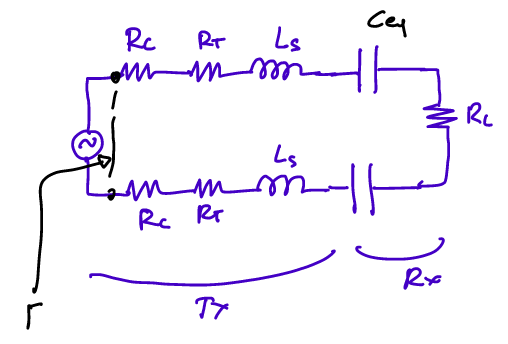
\includegraphics[scale=0.5]{immagini/circ_equiv.png}
	\caption{Circuito equivalente}
\end{figure}\\\\
(ogni resistenza fa riferimento alle perdite!!): il filo è approssimabile bene con l'induttanza in genere, possiamo assumere che le $R_C <<R_T$. C'è una formula che dice che la PTE (rapporto fra la potenza rilasciata sul carico e la potenza in ingresso) è 
\begin{equation}
	PTE = \frac{R_L}{R_L + R_T} (1 - \abs{\gamma}^2)
\end{equation}
e stesso vale per 
\begin{equation}
	R_T = R_L [\dfrac{d}{A \epsilon_0 \epsilon_r}]
\end{equation}
Quindi la PTE complessivamente aumenta se:
\begin{itemize}
	\item  aumenta la A
	\item diminuisce la d
\end{itemize}
quindi elettrodi larghi e dispositivi molto vicini.\\Vediamo come è correlata la massima potenza di tx immissibile nel dispositivo rispetto al SAR: sappiamo che il SAR è limitato: 
$
SAR_{max} =
\begin{cases}
	2 \dfrac{W}{kg} & \text{per testa e addome}\\
	4 \dfrac{W}{kg} & \text{per testa e addome} negli arti
\end{cases}$
Per legare il SAR alla potenza massima:
\begin{equation}
	PTE = \frac{P_L}{P_{TX}}	
\end{equation}
considerando 
\begin{equation}
	P_{TX}(1-PTE)	
\end{equation}
questa è la potenza che viene dissipata nel corpo, ovvero la $P_j$, quindi PTE*P$_{TX}$ è proprio la potenza ceduta al corpo mentre quella dissipata è l'altra.\\Consideriamo 10g di tessuto:

$P_j(10g) = \int\int\limits_{10gr} SAR dm$, ammettendo il SAR costante perché il volume è piccolo, possiamo ottenere $SAR * 10^{-2}$ W, quindi $P_jmax (10gr) = SAR_{max}10?{-2}$ che è la massima potenza che si può rilasciare in una massa di 10g.\\Facciamo un ipotesi brutale: immaginiamo che tutta la potenza venga rilasciata in un paio di cubetti di 10gr, quindi la max potenza rilasciabile in 20g è : $2*10^{-2}SAR_{max}$ che è molto conservativa come ipotesi perché la potenza viene distribuita su un volume maggiore.\\Allora la $P_jmax(20g) = P_{TX}(1-PTE)$ da cui la $P_{TX_{max}} = 2*10^{-2}SAR_{max}/1 - PTE$, quindi se il SAR è 2 $\frac{W}{kg}$ otteniamo un $P_{j_{max}} = \frac{0.04}{1-PTE} W$, nella testa ed addome, mentre negli altri avremmo $\frac{0.08}{1-PTE} W$.\\Quindi se la PTE fosse il 50\%, ma in realtà tipicamente è molto più bassa, avremmo circa 0.1W di P$_{TX}$ che può suonare bene (da quindi un'ordine di grandezza di riferimento).

\subsection{Criticità}
La criticità è simile a quella dell'accoppiamento induttivo ovvero i disaccoppiamenti, i due condensatori tendono a chiudere meno bene le correnti è c'è una perdita di efficienza di trasferimento.\\Il campo lavora su delle discontinuità, quindi nel grasso come ricordiamo (è poco vascolarizzato) c'è maggiore (vedi sopra).\\


\section{Link nel mid-field}
Fin ora abbiamo visto link a frequenze molto basse, aumentandola i dispositivi sono più lontani e non si può più approssimare ad elettrostatico o magnetostatico, siamo quindi nel midfield (regione di Fresnell, non siamo così lontani).\\Quando siamo a frequenza maggiori del GHz, e tipicamente più piccole dei 3GHz le perdite del corpo sono più alte, quindi $\sigma_{body}$ è più alta ma ci spostiamo qui perché se la frequenza è più elevata:
\begin{itemize}
	\item c'è un vantaggio nel bitrate, posso trasmettere informazioni più velocemente
	\item gli oggetti possono diventare elettricamente più grandi e quindi possiamo usare anche più oggetti contemporaneamente e quindi usare degli array di trasmettitori nel corpo
\end{itemize}
\textbf{RICHIAMO}: ciò che comanda nel mondo delle antenne non è la lunghezza l del dispositivo ma la sua dimensione elettrica che è $\frac{l}{\lambda}$ e la lunghezza d'onda nel vuoto è $\lambda_0$ ma in un mezzo con perdite è $\lambda_0/\sqrt{\epsilon_r}$ e quindi se abbiamo aria e sotto un mezzo biologico, se arriva un onda con una certa $\lambda_0$, quando entra nel mezzo la lunghezza d'onda diminuisce perché viene divisa per il valore di permettività del mezzo.\\Quindi all'aumentare della frequenza, siccome $\lambda_0 = \frac{\lambda}{f}$ la lunghezza fisica del dispositivo è 
\begin{equation}
	L_e = \frac{L}{C}f \sqrt{\epsilon_r}	
\end{equation}
quindi abbiamo un dispositivo elettricamente più grande pur rimanendo piccolo, quindi abbiamo un maggiore controllo sul campo EM irradiato.\\La lunghezza EM è 
\begin{equation}
	L_e \propto f\sqrt{\epsilon_r}
\end{equation}
e la frequenza migliore si ha per 1GHz, ovvero l'efficienza di un'antennina impiantata anche tenendo conto delle perdite è quella ottimale e vale nell'ipotesi in cui $D_{IMD} > 1cm$ e si ottiene la frequenza alla quale l'oggetto impiantato risulta efficiente come antenna.\\\\Abbiamo come altro vantaggio di poter usare più di un dispositivo:\\
\begin{figure}
	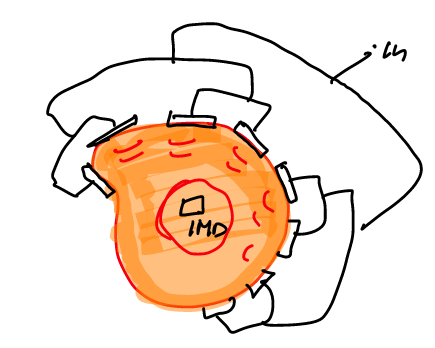
\includegraphics[scale=0.5]{immagini/disp_imp.png}
	\caption{Disposizione di vari dispositivi impiantati sul corpo}
\end{figure}
\\\\possiamo usare vari tipi di trasmettitori all'esterno che, siccome la frequenza è elevata, sono geometricamente piccoli ma elettricamente più grandi.\\Possiamo quindi collegarli con una rete di fascio, mandano un segnale in ingresso posso far si che ciascuno irradi un campo solo nel punto dove serve, quindi per focalizzare l'interrogazione in una piccola regione e si può fare perché gli oggetti sono piccoli geometricamente ma grandi (e quindi posso farli risonanti) elettricamente.\\Il vantaggio è che ognuno produrrà un SAR più basso, riuscendo quindi a rimanere entro i limiti delle normative.\\I conti sono complicati, non possiamo usare i concetti di guadagno delle antenne etc... quindi si introduce un modo di lavorare che non necessita approssimazione ma si rinuncia al rappresentare tutti i fenomeni: introduciamo il \textbf{guadagno di trasduzione}

\subsection{Guadagno di trasduzione (Transducer Power Gain)}
Il guadagno di trasduzione tiene conto di vari fatti ed è specifico per una configurazione particolare.\\Per ottenerlo, dobbiamo rappresentare l'antenna come una rete a due porte: immaginiamo di avere due antenne una che tx ed una che rx\\
\begin{figure}
	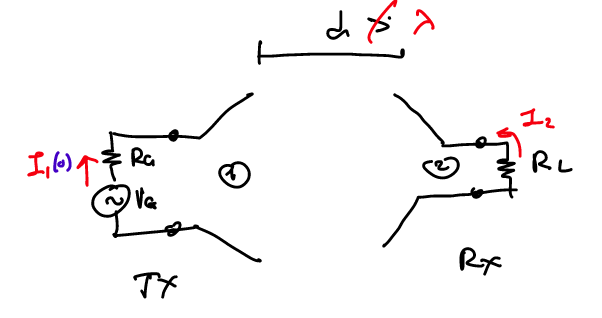
\includegraphics[scale=0.5]{immagini/rete_dp.png}
	\caption{Rappresentazione di un'antenna come rete a due porte}
\end{figure}
\\\\le antenne sono vicine, la distanza d non è più grande di $\lambda$ e quindi c'è disturbo.\\Occorrerebbe fare un calcolo del campo e della tensione raccolta, ma ci interessa analizzare il link di comunicazione, quindi che succede sul carico del ricevitore quando alimentiamo il trasmettitore: immaginiamo di rappresentare tutto come una scatola che verrà analizzata solo ai morsetti\\
\begin{figure}
	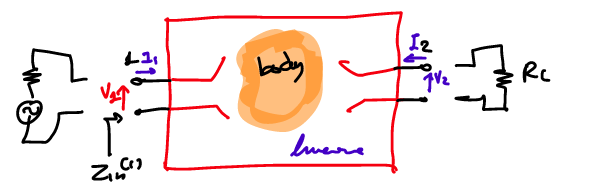
\includegraphics[scale=0.5]{immagini/antenna_scatola.png}
	\caption{Rappresentazione dell'antenna come una "scatola chiusa"}
\end{figure}
\\\\guardando quindi tensione $V_1$ e corrente, che consideriamo entrante nella rete $I_1$ e le $V_2$ ed $I_2$. Non perdiamo nulla perché dipendono dalle interazioni EM che stanno "dentro la scatola", che sono le osservabili.\\Consideriamo che il sistema sia lineare, possiamo immaginare che la tensione che vediamo ad una porta sia $V_1 = I_1$, guarderemo il seguente sistema:
$
\begin{cases}
	V_1 = I_1(0) Z_{11} + Z_{12}I_2\\
	V_2 = I_1(0) Z_{21} + Z_{22}I_2\\
\end{cases}
$
la corrente viene considerata sul punto di alimentazione, da cui la valutazione in 0 (ma la corrente tipicamente scorre ovunque).\\I coefficienti Z sono la \textbf{matrice di impedenza}\\\\
$
\begin{bmatrix}
	Z_{11} & Z_{12}\\
	Z_{21} & Z_{22}\\
\end{bmatrix}
= [Z]
$
\\\\dove i coefficienti sulla diagonale corrispondono al caso in cui si misura la corrente sulla porta 1 quando la porta 2 è in circuito aperto e viceversa, ovvero:
\begin{equation}
	Z_{ii} = \frac{V_i}{I_i}\bigg\rvert_{I_j = 0}
\end{equation}
\\Gli altri due coefficienti sono uguali se la rete è \textbf{reciproca}:
\begin{equation}
	Z_{ij} = Z_{ji} = \frac{V_i}{I_j}\bigg\rvert_{I_i = 0}
\end{equation}
ed sono \textbf{l'impedenza mutua} ed è il termine che da l'accoppiamento fra le due porte.\\L'impedenza in ingresso alla porta 1si esprime come 
\begin{equation}
	Z_{in}^{(1)} = \frac{V_1}{I_1} = Z_{11} + Z_{12}\frac{I_2}{I_1}	
\end{equation}
quindi la dipendenza è mediante il termine di impedenza mutua che da l'accoppiamento, e vale anche il viceversa 
\begin{equation}
	Z_{in}^{(2)} = \frac{V_2}{I_2} = Z_{22} + Z_{21}\frac{I_1}{I_2}
\end{equation}
\\Immaginiamo alcuni casi
\begin{itemize}
	\item[1)] L'antenna rx è chiusa in corto circuito\\
	\begin{figure}
		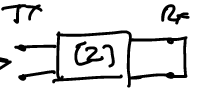
\includegraphics[scale=0.7]{immagini/rx_cortoc.png}
		\caption{Ricevente chiuso in corto circuito}
	\end{figure}
	\\\\L'impedenza che vedo è $Z_{in}^{(1)}$, se $V_2 = 0$ possiamo calcolare 
	\begin{equation}
		\frac{I_2}{I_1} = - \frac{Z_{21}}{Z_{22}}	
	\end{equation}
	e quindi avere  
	\begin{equation}
		Z_{in}^{(1)} = Z_{11} -\frac{Z_{12} \cdot Z_{21}}{Z_{22}} = Z_{11} -\frac{Z_{12}^2}{Z_{22}}	
	\end{equation}
	Quando questo avviene l'oggetto alimentato è fortemente infastidito dalla presenza dell'oggetto non alimentato
	\item[2)] L'antenna rx è in circuito aperto: la configurazione è la seguente\\
	\begin{figure}
		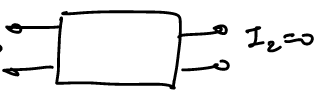
\includegraphics[scale=0.7]{immagini/ric_aperto.png}
		\caption{Antenna ricevente in circuito aperto}
	\end{figure}
	\\\\avremo $I_2 = 0$ e vediamo la $Z_{in}^{(1)}$, dall'espressione di prima viene cancellato un termine e quindi 
	\begin{equation}
		Z_{in}^{(1)} = Z_{11}	
	\end{equation}
	e possiamo dire che l'impedenza in ingresso sia simile a quella dell'antenna se fosse isolata.\\Normalmente in queste condizioni l'antenna tx risente poco della rx (a meno che questa non siamo molto grande).\textbf{IMPORTANTE: la $Z_{11}$ NON rappresenta l'impedenza dell'antenna isolata, ma è molto simile sopratutto se l'antenna ricevente è piccola.}
	\item[3)] Il caso più generale è quando RX è collegato ad un carico $Z_L$, $Z_{in}^{(1)}$ si ricava in quanto esistono diverse rappresentazioni circuitali:
	\begin{itemize}
		\item a $\pi$;
		\item a T
	\end{itemize}
	che hanno le stesse relazioni di grandezze in uscita di una rete a due porte, è dimostrabile (\textsf{\textbf{ma io credo al prof sulla parola}}).\\La rete più semplice è quella a T, una rete a T che ha la stessa matrice di impedenza di una rete a due porte ha questi valori:\\
	\begin{figure}
		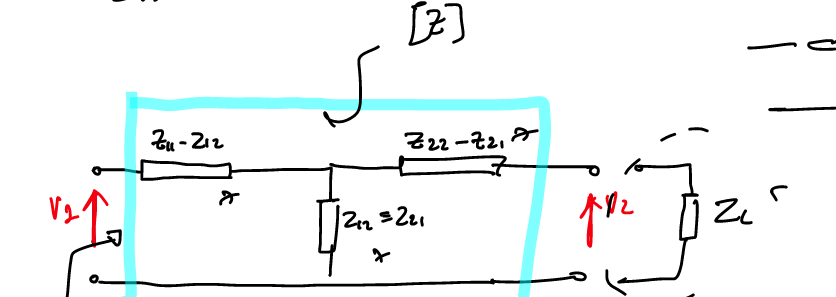
\includegraphics[scale=0.5]{immagini/rete_t_equiv.png}
		\caption{Rete "a T" equivalente alla rete a due porte}
	\end{figure}
	\\\\calcolando l'impedenza in ingresso $Z_{in}^{(1)}$ corrisponde a quella di una rete a due porte.\\Si può fare risolvendo il circuito (che viene lasciato per esercizio?) ottenendo 
	\begin{equation}
	Z_{in}^{(1)} = Z_{11} - \dfrac{Z_{12}^2}{Z_{22} - Z_L}	
	\end{equation}
	\\Se nell'antenna da sola bastava la Z in ingresso qui serve la matrice Z, e questo si chiama impedenza passiva, tiene conto dell'altro oggetto ma non alimentato (se fosse alimentato ci vorrebbe l'impedenza attiva e sarebbe più complesso).
\end{itemize}
Vogliamo esprimere la potenza che viene raccolta dal carico del rx rispetto a quella che viene mandata in ingresso ed (altro) ed introdurremmo il guadagno di trasduzione.\\Ripartiamo dalla rete a due porte, che rappresentiamo con la matrice di impedenza\\
\begin{figure}
	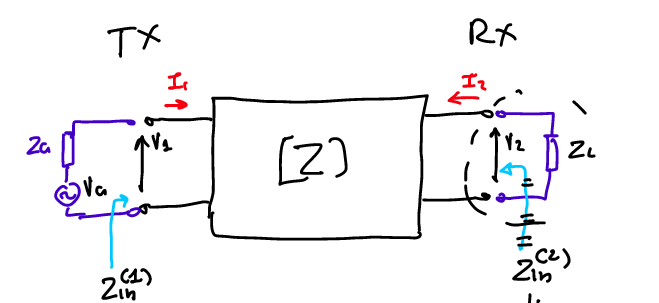
\includegraphics[scale=0.5]{immagini/rete_dp_matr.png}
	\caption{Rete a due porte con matrice d'impedenza}
\end{figure}
\\\\possiamo quindi vedere le impedenze in ingresso alle diverse porte del tx e dell'rx, sappiamo che sono date da:
\begin{equation}
	Z_{11}^{(1)} = Z_{11} - \frac{Z_{12}^2}{Z_{22}+Z_L}	
\end{equation}
e 
\begin{equation}
	Z_{22}^{(2)} = Z_{11} - \frac{Z_{12}^2}{Z_{11}+Z_G}	
\end{equation}
Vediamo l'equivalenza di Thevenhin:\\
\begin{figure}
	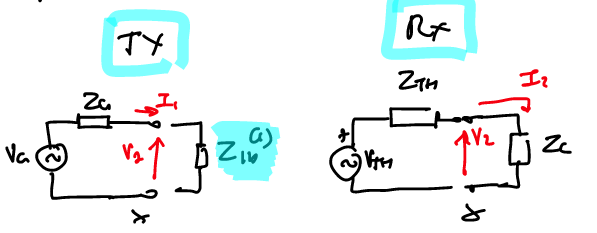
\includegraphics[scale=0.6]{immagini/equiv_thev_rx_tx.png}
	\caption{Equivalenza di Thevenhin per rx e tx}
\end{figure}
\\\\guardando da sinistra, un'osservatore vedrà tutto quello che accade dentro dal valore di $Z_{11}^{(1)}$ e questo è per il tx, mentre per l'rx: ci saranno impedenza di Thevenhin e generatore di Thevenhin che vanno calcolate.\\Possiamo quindi studiarli separatamente, nel secondo valuteremo la potenza che verrà distribuita sul carico.\\Partiamo dalla $Z_{Th}$ che è l'impedenza passiva che vediamo verso l'interno avendo staccato il generatore, quindi è uguale all'impedenza di ingresso che avremmo calcolato con il circuito attivo 
\begin{equation}
	Z_{Th} = Z_{in}^{(2)}	
\end{equation}
\\La tensione del generatore è data dal fatto che il circuito è aperto, riprendiamo l'espressione di $V_2$ circuitale 
\begin{equation}
	V_2 = Z_{21}I_1	
\end{equation}
in quanto il termine con $I_2$ È 0 perché i circuiti sono staccati.\\Esplicitiamo
\begin{equation}
	V_1 = V_{C1} - Z_G I_1 \equiv Z_{11}I_1 + Z_{12}I_2\bigg\rvert_{I_2 = 0}
\end{equation}
sapendo che $I_2$ = 0 avremo 
\begin{equation}
	I_1 = \dfrac{Z_G}{Z_{11} + Z_G}	
\end{equation}
Inseriamo l'espressione trovata per trovare la 
\begin{equation}
	V_{Th} = V_2 = \dfrac{Z_{21}}{Z_{11} + Z_G} V_G	
\end{equation}
Ora possiamo usare i due circuiti per fare delle considerazioni di potenza: consideriamo 2 potenze
\begin{itemize}
	\item $P_L$, che il trasmettitore rilascia al carico del ricevitore.\\È data da 
	\begin{equation}
		P_L = \frac{1}{2} R_{L}|I_2|^2	
	\end{equation}
	è quella che serve al dispositivo impiantato per farlo funzionare. La $I_2$ si ricava da
	\begin{equation}
	I_2 = \dfrac{V_{Th}}{Z_{in} + Z_L}	
	\end{equation}
	quindi
	\begin{equation}
		P_L = 
		\frac{1}{2} \dfrac{\abs{Z_{21}}^2 \abs{V_G}^2 R_L}{\abs{Z_{11} + Z_G}^2} \dfrac{1}{\abs{Z_{22} - \frac{(Z_{21}^2)}{Z_{11 + Z_G}} + Z_L}^2}
		= \frac{1}{2} \dfrac{\abs{Z_{12}}^2 \abs{V_G}^2 R_L}{\abs{(Z_{11} + Z_G)(Z_{22}+Z_L) - Z_{12}^2}^2}
	\end{equation}
	\item $P_{in}^{(1)}$ che è quella che entra nell'antenna trasmittente data da 
	\begin{equation}
		P_{in}^{(1)} = \frac{1}{2}R_{in}^{(1)} |I_1|^2 
	\end{equation}
	In particolare 
	\begin{equation}
		P_{in}^{(1)} = \frac{1}{2}R_{in}^{(1)} \dfrac{\abs{V_G}^2}{\abs{Z_{11} + Z_G}^2}
	\end{equation}
\end{itemize}
Definiamo ora la \textbf{potenza disponibile} in ingresso (available power) che è la $P_{AV,G}$ che è la massima potenza che il generatore può erogare verso la rete e che viene erogata nelle condizioni in cui l'impedenza delle rete è il complesso coniugato dell'impedenza del condensatore 
\begin{equation}
	Z_{in}^{(G)} = Z_G^*	
\end{equation}
(adattamento coniugato, $R_{in}^{(1)} = R_G$ e $X_{in}^{(1)} = -X_G$)
quindi 
\begin{equation}
	P_{AV,G} = \dfrac{\abs{V_G}^2}{8R_G}	
\end{equation}
Qualcosa del genere si fa in uscita ed è la \textbf{network available power}, che è la massima potenza che la rete è in grado di rilasciare al carico e si ha la massima quando l'impedenza in ingresso in 2 è uguale al complesso coniugato della $Z_L$.\\Vale 
\begin{equation}
	P_{AV,N} = max{PL} = \dfrac{\abs{V_{Thev}}^2}{8 R_{Th}}	
\end{equation}
Definiamo finalmente il $G_T$ (transducer power gain) uguale per definizione a
\begin{equation}
	G_T \triangleq \frac{P_L}{P_{AV,G}} 	
\end{equation}
ed è importantissima perché dipende dal fatto che rx non è adattato al carico, che c'è un mezzo con perdita etc... e la dobbiamo ottimizzare perché sappiamo che
\begin{equation}
	P_L = P_{AV,G} G_T	
\end{equation}
sostituendo nella precedente viene fuori la relazione
\begin{equation}
	G_T = \dfrac{4R_G R_L \abs{Z_{12}}}{\abs{ (Z_{11} + Z_G) (Z_{22} + Z_L) - Z_{12}^2}^2}
\end{equation} 
(che è adimensionale essendo un guadagno). (N.B: la X è la reattanza).È la grandezza da tenere in conto quando si progetta il sistema.


\chapter{Lezione 7}
\section{Ancora sul guadagno di trasduzione}
Possiamo scrivere la potenza che finisce sul carico $P_L$, che è quella che serve al dispositivo se non ha una batteria per accendersi: come $P_L \equiv P_{R\rightarrow T} P_{AV,G} G_T$, dove $G_T$ è specifica della configurazione, quindi se ad esempio ruoto un dispositivo rispetto all'altro devo ricalcolare il guadagno di tr asduzione.\\In ingegenria è solito calcolare il margine, che è la \textbf{capacità di dormire la notte}, ovvero avere della capacità in più per le evenienze: $p_0$ è la minima potenza da rilasciare sul carico tale per cui il ricevitore funzioni, ovvero la $min\{P_L\}$, il margine in scala linerare è : $M = \frac{P_L}{p_0}$ dove $p_0$ è la power sensitivity.\\Se la quantità è $<$ 1 stiamo rilasciando una potenza più piccola di quella che serve al dispositivo per funzionare, quindi non avremo il link, mentre pi è maggiore di 1 e più il link è robusto.\\Normalmente si rappresenta in DB: $M_{db} = P_{AV,G} + G_T -p_0 - M_0$ dove $M_0$ è un margine aggiuntivo che cerca di tenere conto di eventuali difetti fisici dell'oggetto per cui conta che viene mantenuta della potenza in più.\\Il radio collegamento si stabilisce quando $M_{db} > 0$, quindi più è grande più si compensano fenomeni di cui non si era tenuto conto durante il progetto.\\\textbf{Con margine pari a 0 ce dice bene se funziona na volta sola a culo}, mentre invece con della potenza di riserva c'è una sicurezza maggiore.\\esempio: (copia disegnino) la linea rappresenta la sensitivity + margine aggiuntivo, quindi dire che $M_{db} > 0$ vuol dire che $P_{AV,G} + G_T > p_0 + M_0$. Se abbiamo progettato bene il dispositivo il picco sarà sulla frequenza di lavoro $f_0$, avremo quindi una regione dove c'è il collegamento ed una dove non c'è.\\Il grafico si fa spesso rispetto anche ad un parametro di progetto, come ad esempio la dimensione, la freccia viola indica quanto si è sicuri che il dispositivo sia robusto rispetto a delle cose che non si è riusciti a prevedere.\\Fissata la potenza in ingresso (che è strettamente finita) occorre progettare i dispositivi al meglio possibile in modo che $G_T$ sia elevato.
\subsection{Guadagno di sistema}
(Orfanidis, pdf free: libro di EM dove nel cp 5 c'è questa parte).\\IL guadagno di sistema è definito come:
\begin{equation}
	g = \dfrac{\text{max}\{P_L\}}{\text{Potenza entrante nella rete} (P_in)}
\end{equation}
dove la massima $P_L$ è quella che abbiamo chiamato la $P_{AV,n}$.\\Questa espressione differisce da quella di prima in quanto presuppone l'adattamento coniugato in ingresso ed in uscita, uqinid è il caso migliore: se il trasponder venisse progettato perfettamente adattato ripsetto a ciò che vede in ingresso e l'interrogatore perfetto rispetto a ciò che arriva dall'esterno avrei questo massimo:\\
$Z_{in}^{(1)} = Z_{G}^*$ (copia)
moltiplicando: (copia) otteniamo l'upper bound per il link.\\ \textbf{Perché è importante:} quando si fa un progetto, non si "spacca subito il capello" se magari ci sono molti parametri, quindi se il link va progettato secondo certe condizioni ci si chiede se occorre progettare l'antenna proprio così.\\Posso assicurare che le due antenne riescano a comunicare? Quello che si fa è fare un design di massima senza preoccuparsi di adattare subito le antenne, ma messe in un certo modo nel caso migliore si riesce a tx una potenza sufficiente da poter fare accendere l'antenna rx? Allora controllo il guadagno di sistema, se mi ci trovo e quindi il margine è sufficiente per lavorare, allora penso a poter ottimizzare le antenne per poter lavorare.\\Il calcolo si ottiene mettendo le espressione trovate prima:
\begin{equation}
	g = \dfrac{\frac{1}{8}\frac{\abs{V_{Th}}^2}{R_{Th}}}{\frac{1}{2} \dfrac{\abs{Z_{12}}^2 R_L \abs{V_G}^2}{\abs{(Z_{11}+Z_G)()}^2}}
\end{equation}
(copia)\\Esiste poi un'espressione molto pulita se si fa riferimento alla \textbf{matrice di scattering}, "cugina" della matrice di impedenza, ovvero è una rappresentazione con un'onda di tensione che entra che è $a_1$ ed un'onda di tensione che torna indietro (l'onda riflessa dall'interfaccia) $b_1$ ed anche le $A_2, B_2$ dove $V_1$ e $V_2$ in funzione di A:
\begin{equation}
	V_1 = \sqrt{Z_0}(a_1 + b_1)
\end{equation}
si può anche trovare una relazione matriciale, ($Z_0$ è l'impedenza di riferimento della linea. Tipicamente, se il carico non è complesso, sono 50$\Omega$) e la matrice di scattering è tale per cui:\\ (copia) per capirci l'$S_{11}$ corrisponde al coefficiente di riflessione della porta 1 isolata dalla 2.\\Otteniamo quindi un'espressione del guadagno di sistema: (slides)\\\\\textbf{Esempio:}\\
immaginiamo di avere un moncherino di un braccio, nel quale siano stati impiantanti dei sensori miografici che raccoglie gli impulsi della mano che si apre/chiude (\textbf{perché il muscolo lo ricorda :O}). Immaginiamo di mettere due sensori A e B e sopra l'antenna TX (immagini), si usano due sensori perché si acquisisce il segnale del muscolo agonista ed antagonista. I due dispositivi sono a differenti profondità rispetto al TX e quindi daranno guadagni di trasduzione diversi.\\Immaginiamo di aver calcolato i guadagni di trasduzione, troviamo questa situazione:
\begin{table}
	\begin{tabular}{|c|c}
		 & G[DB]\\
		 \hline
		 A & -15\\
		 B & -25\\
	\end{tabular}
\end{table}
$p_0 = -15 dBm$, dove x dbM = xdB - 30, quindi se 1W = 0dB $\rightarrow$ 1W = 30dbM (1W = 1000 mW)\\$M_0 = 3dB$, cerchiamo la $P_{av,G}$ per attivare il link fra i due dispositivi.\\Abbiamo visto che $P_{av,G} + G_T > p_0 + M_0$, $P_{av,G} > -G_T + p_0 + M_0$. Riconduciamo alla stessa unità di misura poi:
\begin{itemize}
	\item[A] $P_{av,G} = -15dBm + 3dB + 15dB$. Portiamo tutto in dBm, riscriviamo $P_{av,G} = M_0\frac{p_0}{G_T}$, vanno espressi $p_0$ e $G_T$ o in W o in mW. Quindi, in dB: -45dB +3dB +15dB = -27dB, che sono 3dBm ovvero 2mW.
	\item[B] +25dB -15 dbM +3dB.\\Riportiamo tutto in dB, +25dB (-15-30)dB + 3dB = -17 dB. Conviene riportare tutto in DB visto che il margine aggiuntivo è espresso in dB.
\end{itemize}
\subsection{Link asimmetrico - guadagno di Round-Trip}
Consideriamo di avere un ricevitore RX che sia privo di sorgente e per comunicare con il trasmettitore deve usare la modulazione del segnale di interrogazione (simile a ciò che avviene nei link induttivi).\\Prendiamo il circuito di Thevenhin del RX: (immagine), immaginiamo che nella modalità in cui $TX \rightarrow RX$ il carico venga collegato ad uno switch che in base ad una logica binaria, se si vuole trasmettere 1 o 0, commuta su uno dei due carichi.\\I due carichi sono molto diversi, quindi normalmente $Z^{OFF} >> Z^{ON}$.\\I due dispositivi sono accoppiati, quindi il trasmettitore si accorgerà che dall'altra parte sta cambiando qualcosa: (rifare schema della rete a due porte).\\Il coefficiente di riflessione che il reader vede è dato da (copia)\\
l'impedenza tramite $Z_in^{(1)}$ è funzione del particolare stato di commutazione del carico.\\Si può far vedere che ci sono segnali sinusoidali che vengono trasmessi, rimuovendo la portante si vede che la potenza che il trasponder manda indietro al reader si scrive come (nb ci sono delle gamme) (copia) quindi dipende dalla potenza massima iniettata nella porta moltiplicata per una grandezza che dipende dai valori di impedenza.\\Valori tipici:
$Z^{OFF} \rightarrow \infty$
$Z^{ON} \rightarrow Z_L$.\\Quindi come caratterizzaimo il link andata e ritorno: introduciamo il guadagno di Round-Trip definito come:
\begin{equation}
	G_{RT} = \frac{P{R \leftarrow T}}{P_{a, G}} = \frac{1}{4} [\Gamma_{in}^{(1)} (Z^{ON}) - \Gamma_{in}^{(1)}(Z^{OFF})]^2
\end{equation}
che è data da (copiare e mettere da parte) dove deve valere la condizione: (copia) per stabilire il link totale inverso.\\Possiamo anche qui definire una margine di Round-Trip (in dB siamo in scala 10$log_{10}$): (copia) quando la quantità è $\geq 10$ abbiamo che il link inverso è attivato.(copia disengo): c'è il segnale che va dal reader al transponder e poi dal transponder torna indetro e viene raccolto dal reader. Abbiamo quindi due margini:
\begin{itemize}
	\item per il link diretto (copia)
	\item per il link di Round-Trip
\end{itemize}
quindi il link è stabilito quando ambe due le grandezze sono maggiori di 0, altrimenti può accadere che accendo il transponder ma questo risponde "debolmente" o viceversa.\\Tipicamente qui il bottleneck è l'$M_D$ perché tipicamente la sensitivity del transponder è molto più "scarsa", specialmente se questo è senza batteria.\\Se il link diretto è verificato ho quindi buone possibilità che lo sia anche quello inverso (ma non è sempre così).\\\\In generale, $G_{RT} << G_T$ perché nel primo caso c'è un'attenuazione dovuta al fatto che entra e poi torna indietro quindi se il mezzo è con perdite subisce due forti attuazioni invece di una sola.\\\\La maggior parte di questi link funziona posizionando il lettore sul corpo e leggendo dal dispositivo impiantato. Ci sono dei casi in cui c'è vantaggio a leggere il dato da fuori, ad esempio protesi che monitorano le infezioni in modo che ad esempio un lettore che è in bagno legga il dato per individuare i precursori dell'infezione.\\Ovviamente si è esposti ad attacchi malevoli.

\section{Link in campo lontano}
Qui valgono tutte le grandezze inserite studiando le antenne classiche. Questo tipo di link si ha tipicamente quando abbiamo dispositivi wearable che comunicano con l'esterno: (immagine) abbiamo il corpo ed immaginiamo che il dispositivo sia o all'esterno o anche all'interno ma venga interrogato a distanza.\\Abbiamo il reader (interrogatore) e la distanza d è tale per cui ogni oggetto è nel campo lontano dell'altro, da cui il limite di Foun... $r_F \geq \frac{2D^2}{lambda}$.\\Per il reader, $d > \frac{D_r^2}{\lambda}$, dove $\lambda_0$ è sempre quello nel vuoto.\\Per il dispositivo sul corpo, la dimensione che conta è quella dove c'è della distribuzione di corrente ovvero dove il corpo diventa un pezzo dell'antenna. quindi $d > \frac{D_{MD}^2}{\lambda_0}$ dove immaginiamo una zona dove ci sono delle correnti di conduzione che possono a loro volta produrre delle radiazioni.\\In queste condizioni, possiamo studiare i due oggetti separatamente per poi metterli assieme con le regole di campo lontano: (copia immagine)\\
il trasmettitore sarà caratterizzato da guadagno e potenza entrante mentre il ricevitore dal guadagno e dalla potenza rilasciata sul carico, allora $P_{RX} = P_{TX} G_{TX} G_{RX} \tau_{TX} \tau_{RX} (\frac{\lambda4\pi d})^2 \eta_p$
dove $\tau_{TX}$ (?) oppure vale $4\pi \dfrac{R_{TX} R_G}{\abs{Z_{TX} + Z_G}^2}$
mentre $\tau{RX}$ (copia) e valgono 1 quando c'è adattamento coniugato: (copia).\\I prodotti sono il guadagno realizzato $\tilde{G}_{TX}$ di TX ed RX (rx tiene conto del fatto che non tutta la potenza raccolta può essere trasferita al carico perché può esserci del disallineamento).\\ La eta tiene conto di come sono allineate la polarizzazioni fra le due antenne (efficienza di polarizzazione), matematicamente: (copia). Il termine $(\frac{\lambda_0}{4 \pi d})^2$ è l'attenuazione di spazio libero, quindi la densità di potenza si attenua per volumi più grandi in quanto si distribuisce man mano che ci allontaniamo su sfere più grandi.\\Il $^2$ vale solo per lo spazio libero, altrimenti ci sarà un valore più altro se ci sono riflessioni da terreno pareti etc...


\chapter{Lezione 8}
\section{Far field - link simmetrici}
Abbiamo considerato il link diretto, dove abbiamo che i due dispositivi sono posti a distanza grande rispetto alla distanza di (fonofer scopri come se scrive).\\Continuiamo con link diretti, ricaviamo dalla formula di fris la distanza massima del collegamento: introduciamo una p del ricevitore che è la power sensitivity del ricevitore: se $P_{rx} \geq p_{rx}$ allora li link sarà attivo altrimenti non si stabilisce.\\Considerando l'uguaglianza, possiamo trovare la distanza massima con cui tale collegamento si stabilisce: $P_{rx} = p_{rx}$. facciamo Fris$^{-1}$ e trviamo che $d_{max} = \frac{\lambda}{4\pi} \sqrt{\dfrac{G_{TX} P_{TX}G_{RX}\tau_{TX} \tau_{RX}}{p_{rx}} \eta}$. Se abbiamo adattato il tx, abbiamo una proporzionalità (copia) e se anche il ricevitore è fissato abbiamo prop. com (copia).\\In dB, avremo che $d_{max} \propto \frac{1}{2} G_{RX}$, sappiamo che 3dB è circa un 2x di guadagno, ogni 6dB (4 volte di guadagno) si ha un raddoppio della distanza del link (la radice la porta a 2).\\Invece, un aumento di guadagno di 3dB dice che òa distanza di lettura aumenta di un fattore $\sqrt{2}$ (circa 1 volta e mezza) (IMPORTANTE).\\Facciamo un grafico questo concetto: (copia grafico)\\c'è un'attenuazione che andrebbe come $(\frac{d}{\lambda})^{-2}$. Avendo quindi fissato il sistema di lettura, un modo per aumentare la distanza è cercare di abbassare la sensitivity (ma ci sono i limiti fisici ad un certo punto).\\Per link simmetrici vale la stessa cosa, basta invertire rx con tx, in questo caso il trasponder è dotato di una sorgente locale di alimentazione.
\section{Far field - link asimmetrici}
Qui i ruoli fra transponder ed interrogatore non si scambiano mai, applicheremo quindi nuovamente un protocollo di modulazione dell'impedenza, ma non nell'accoppiamento bensì nel back scattering (riflessione).\\Immaginiamo la seguente situazione: (copia disegno)\\la distanza d è di campo lontano, il reader avrà un suo guadagno $G_R$ ed anche il transponder $G_T$.\\Il reader manderà un segnale ed il transponder lo andrà a riflettere modulandolo: avremo un vettore di Pointing dal transponder verso il reader e poi ci sarà un giro di round trip indietro, abbiamo un fenomeno di \textbf{scattering}, che verrà pilotata dal carico.\\Questo è il classico modello radar, dove c'è un antenna che manda impulsi verso un aereo ma qui la differenza è che il segnale che torna indietro deve portare informazione ovvero una sequenza binaria.\\Scriviamo la densità di potenza $S_{R \rightarrow T}(d) = \frac{1}{2Z_0}\abs{E_{R \rightarrow T}(d)}^2$ che si può anche scrivere come (copia) dove la I è l'intensità di radiazione che è densità di potenza per unità di angolo solido.\\Entra in gioco nel guadagno dell'antenna trasmittente: $G_R = \frac{I_R 4\pi}{P_R}$ da cui possiamo ricavare $P_R = \frac{P_{in}G_R}{4 \pi}$, la inseriamo nell'espressione della densità di potenza ottenendo $S_{R \rightarrow T}(d) = \frac{P_{in}G_R}{4 \pi d^2}$ che ci dive come si attenua la potenza man mano che ci si allontana da una sfera di raggio d (o diametro?).\\Introduciamo ora il concetto di \textbf{radar cross-action}: è l'area di uno scatteratore isotropico (riflette allo stesso modo in tutte le direzioni), quindi una sferetta metallica, che una volta investita dal campo retro-diffonde nella direzione dove c'è il mio oggetto la stessa quantità di potenza.\\È la $\sigma$, che va valutata in campo lontano ($d \rightarrow \infty$) $\sigma \lim\limits_{r \rightarrow \infty} 4 \pi r^2 $(copia).\\Utilizzo: conosciamo il campo incidente, possiamo quindi calcolare il campo che emerge dal transponder e torna indietro dal ricevitore: (copia).\\È la potenza $S_{R \rightarrow T}(d)$ e che quindi porterà il segnale che torna indietro.\\La potenza rilasciata sul carico del ricevitore sarà uguale : $S_{R \rightarrow T}(d) \cdot A_{C,R}$ dove $A_C$ è l'area efficacie del reader, ovvero una superficie equivalente che se investita da un'onda raccoglie una quantità di potenza uguale da quella che avrebbe raccolto l'antenna (ed è più piccola dell'area geometrica) (?? vedi bene).\\Mettendo quindi tutto dentro: (copia)\\ci aggiungiamo $\eta_P$ (polarization loss factor) perché se abbiamo un oggetto di una certa forma ed irradiamo con un campo, per effetto della forma probabilemnte il campo scatterato avrà una forma differente, quindi quando incide sull'antenna può non avere la stessa polarizzazione di quando è partito e quindi si tiene in conto con questo fattore. (copia)\\Questa è l'equazione del radar, dipende anche dalla capacità di scatterare del transponder in una direzione rispetto che in un'altra.\\Abbiamo anche che $\sigma$ può essere considerata in due casi:
\begin{itemize}
	\item monostatica: il segnale è raccolto dalla stessa antenna che interroga
	\item bistatico: abbiamo due antenne, una illumina il bersaglio ed un'altra prende il segnale retro-diffuso (tipicamente c'è un vantaggio per quanto riguarda la qualità del segnale)
\end{itemize}
ragioniamo con situazione monostatica:\\la potenza che torna indietro è $\propto \frac{1}{d^4}$ perché deve fare un round trip quindi abbiamo due attenuazioni da $\frac{1}{d^2}$ quindi il segnale retrodiffuso è molto flebile rispetto ad un oggetto che sta trasmettendo di suo.\\Dobbiamo ora fare in modo che arrivi dell'informazione: occorre intanto isolare il dispositivo da tutto il riflesso dell'ambiente. Questo si ottiene con la modulazione, in modo che il segnale che si sovrappone al disturbo oscilli.\\Passiamo ad un'antenna che abbia un'impedenza d'ingresso $Z_a$ ed un carico $Z_L$ con un generatore equivalente che tiene conto del campo che arriva, possiamo esprimere $\sigma$ come $\frac{\lambda^2}{4 \pi} G \abs{A - \Gamma^*}^2$ quindi è lo scattering di un dispositivo caricato.\\$\Gamma^*$ è un coefficiente di riflessione generalizzato, dato dal coefficiente che vedo fra l'antenna ricevente ed il suo carico. Ha come differenza rispetto al classico che c'è un complesso coniugato, perché c'è qualcosa che deve immagazzinare energia.\\ A è un complesso che dipende da forma e soprattutto dimensione dell'antenna scatterante: se la dimensione di tale antenna è $L << \lambda$ allora $A \simeq 1$. In queste condizioni la $\sigma$ del transponder sarà data da: (copia, più passaggi) ottenendo $\sigma_T = \frac{\lambda^2}{4 \pi} G_T^2 $(copia) aggiungiamo di nuovo l'efficienza di polarizzazione perché l'oggetto può cambiare la polarizzazione.\\Questa è quindi l'area di scattering equivalente con un guadagno $G_T$ ed una certa impedenza del carico, che  quella che possiamo variare per far variare l'RCS: possiamo quindi controllare quanto questo oggetto rifletta, se lo facciamo on due stati cambia l'informazione che torna indietro e quindi possiamo mandare informazione.\\Abbiamo che $P_{R \rightarrow T} = (\frac{\lambda}{4 \pi d})^4 P_{in} G_R^2 G_T^2 \dfrac{4 R_{in,T}^2}{\abs{Z_L + Z_{IN,T}}^2} \eta_P^2$ ci interessa che l'equazione sia dominabile andando ad agire sull'impedenza del carico.
\subsubsection{Modulazione di impedenza}
Immaginiamo di avere due stati:
\begin{itemize}
	\item 0, associato ad un'impedenza di carico che sia virtualmente un circuito aperto $Z_L \rightarrow \infty$, e quindi $P_{R \rightarrow T} = 0$
	\item per lo stato 1 si può scegliere: $Z_L = 0$ (corto circuito) che ci da (copia) una potenza $\neq 0$
\end{itemize}
così possiamo cambiare a piacimento la potenza retro diffusa.\\Una scelta di questi due livelli ha un grosso limite: l'oggetto comincia a riflettere ciò che arriva, ma se il RX switcha fra $\infty$ e 0, l'aspetto critico è che, funzionando solo con l'energia che arriva da lontano, non raccolgo quindi potenza: non c'è un carico collegato, quindi la corrente raccolta non può essere immagazzinata.\\Conviene quindi che uno dei due stati sia compresa fra $0$ ed $\infty$, quindi prendiamo $Z_L = Z_{IN,T}^*$ dove quindi in questo stato assorbe e immagazzina energia, mentre nell'altro caso no: (copia) non c'è più dipendenza fra le impedenze. Quindi, nel caso 1 non abbiamo carica remota per il dispositivo, perché non è in grado di raccoglierla.\\Vediamo ora come avviene effettivamente la comunicazione: (copia immagine) abbiamo poi gli altri oggetti che saranno di dimensioni sicuramente più grandi di quelle di tx ed rx. Quando tx produce il suo campo, immaginiamo un'onda continua che si distribuisce in varie direzioni avremo una riflessione non modulata, quindi la stessa sinusoide con la stessa frequenza (attenuata) che finirà sull'rx e poi l'effetto prodotto dalla modulazione di impedenza: (copia disegno) abbiamo quindi nel carico del transponder nuovamente uno switch che connette due stati.\\Avremo quindi l'inviluppo con dentro l'onda che viene riflessa: ha la stessa frequenza del reader ma è modulata in ampiezza.\\Sul reader ci sarà la somma delle onde blu e rosse, l'ambiente grande rifletterà molto di più dell'oggetto che trasmette: (copia altro disegno) ai capi del transponder vedremo quindi un qualcosa del genere: (copia ulteriore disegno) avremo quindi il segnale totale al reader, tolta la sinusoide rimane l'inviluppo e possiamo estrarre il valore inviato.\\Si chiama \textbf{modulazione di back scattering}, che è la tecnologia con cui funzionano tutti i sistemi di identificazione in radiofrequenza.\\Per la distanza massima del collegamento, dobbiamo tenere conto che 
\begin{itemize}
	\item il link diretto,governato dalla formula di Friis serve ad accendere ed alimentare il transponder. Questo va come $(\frac{d}{\lambda})^2$ e si attiva quando (copia)
	\item il link inverso, che va da transponder a reader e serve a modulare il backscattering (copia anche qui)
\end{itemize}
il link si stabilisce quindi quando sono verificate ambe due le condizioni. Anche qui facciamo un grafico per capire la distanza massima del collegamento: (copia disegno)\\ dove $p_R << p_T$ in quanto $p_R: -100dBm - -70 dBm$ mentre $p_T: -20 dBm - -5 dBm$, avremo quindi che $\d_{max} = min\{d_D, d_I\}$ tipicamente il bottleneck è il link al quale compete la lunghezza più breve che è quasi sempre il link diretto.
\subsection{Logica di modulazione}
Cosa c'è nel transponder per acquisire energia e pilotare il transponder alto/basso: c'è una logica di modulazione che ha delle parti analogiche e delle parti digitali.\\Lo schema è il seguente: (copia immagine)\\
la prima cosa che avviene è un passaggio da analogico a digitale, c'è un rettificatore (immaginiamo un diodo collegato ad un condensatore, come se fosse la batteria virtuale del dispositivo) si passa quindi da AC a DC, la corrente alimenterà i componenti, primo fra cui il modulatore.\\Il modulatore comanda il carico e lo fa aprire o chiudere fra due valori, la frequenza a cui vengono fatte queste operazioni è tipicamente più bassa della $f_0$ di interrogazione: c'è un clock che scandisce tale frequenza, quindi anche il segnale di clock serve per gestire il modulatore. Abbiamo poi la RAM che mantiene l'informazione, da cui si legge e su cui si scrive.\\Tutta l'attività è svolta da un circuito integrato che è molto piccolo (chip da 0.5mm - 3mm)\\La prima parte è analogica dove avviene l'energy harvesting, ovvero il raccogliere l'energia, poi c'è il blocco di data modulation ed infine il data access che sono parti digitali.\\Il blocco analogico mette in contatto col mondo esterno, quello digitale serve per fare le operazioni.\\Da un punto di vista a radio frequenza, ci interessa la $Z_L$ per fare i calcoli di adattamento: vedremo l'impedenza del primo blocco analogico: avremo una parte reale dovuta alle perdite e poi un condensatore che serve ad immagazzinare l'energia che arriva da fuori, che può essere serie o parallelo (copia disegno), avremo che $Z_C = R_{IC} - \frac{1}{j \omega C_{IC}}$ dove la parte $R_{IC}$ (copia) è quindi questo il circuito a cui l'antenna di deve adattare per avere un $\tau_T = 1$, deve avvenire che (copia), quindi l'antenna deve essere progettata per lavorare non in risonanza (induttanza ?), sarà l'insieme ad essere risonante.

\chapter{Lezione 9}

















\part{Parte Localization}








\part{Parte Hardware}









































\end{document}
